% Springer Nature (sn-jnl) version, for submission to Mathematical Geosciences.
%
% REQUIRES the official Springer Nature LaTeX template, NOT on CTAN/TeX Live:
%   download "LaTeX template (zip)" from
%   https://www.springernature.com/gp/authors/campaigns/latex-author-support
%   (or the Overleaf "Springer Nature article" template), and place in this
%   folder at least:  sn-jnl.cls  and the reference style sn-basic.bst
%   the reference style sn-mathphys-ay.bst (Math & Physical Sciences,
%   author-year --- the style used by Mathematical Geosciences).
%
% The section files in sections/ are class-agnostic and are shared verbatim
% with main.tex (the generic article draft that compiles without the class).
\documentclass[pdflatex,sn-mathphys-ay]{sn-jnl}

% sn-jnl loads amsmath, amsthm, graphicx, hyperref, natbib (but not amssymb).
\usepackage{amssymb}
\usepackage{mathtools}
\usepackage{bm}
\usepackage{xcolor}
% Tracked changes for revision R1: ... inline, revblock for paragraphs.
% For the clean copy, redefine \revtext to expand to its argument uncoloured.
\newcommand{\revtext}[1]{\textcolor{blue}{#1}}
\newenvironment{revblock}{\par\begingroup\color{blue}}{\endgroup\par}
\usepackage{algorithm}
\usepackage{algpseudocode}
\usepackage{booktabs}

% theorem-like environments
\theoremstyle{plain}
\newtheorem{proposition}{Proposition}
\theoremstyle{definition}
\newtheorem{property}{Property}
\newtheorem{definition}{Definition}
\newtheorem{assumption}{Assumption}
\theoremstyle{remark}
\newtheorem{remark}{Remark}

% notation shortcuts (shared with main.tex)
\newcommand{\R}{\mathbb{R}}
\newcommand{\Z}{\mathbb{Z}}
\newcommand{\E}{\mathbb{E}}
\newcommand{\Prob}{\mathbb{P}}
\newcommand{\norm}[1]{\lVert #1 \rVert}
\newcommand{\neff}{n_{\mathrm{eff}}}
\newcommand{\dip}{\mathrm{dip}}
\DeclareMathOperator*{\argmin}{arg\,min}
\DeclareMathOperator*{\argmax}{arg\,max}

\begin{document}

\title[ESS-calibrated test of cluster homogeneity]{%
Effective-sample-size calibration of a modality test for cluster homogeneity
and the number of classes in spatially autocorrelated data}

\author[1]{\fnm{Francisco} \sur{Parra}}\email{francisco.parra.o@usach.cl}
\affil[1]{\orgname{Universidad de Santiago de Chile},
  \orgaddress{\city{Santiago}, \country{Chile}}}

\abstract{%
Selecting the number of clusters $K$ is a basic step in unsupervised
classification. \revtext{The standard internal criteria, namely the gap statistic,
the average silhouette and the Calinski--Harabasz and Davies--Bouldin indices,
take no account of the dependence between observations. On spatial
data, they therefore leave one question unanswered: whether an apparent
grouping reflects discrete classes or is already produced by the
autocorrelation of a single class.} Because neighbouring locations are
correlated, a scene carries far less information than its pixel count
suggests, and a smooth large-scale trend mimics discrete structure.
\revtext{The effect is systematic: on autocorrelated fields simulated without
discrete classes, these criteria report more than one class in every one of
$75$ realisations. On real imagery, they divide single land-cover regions.}
\revtext{We recast the choice of $K$ as a recursive homogeneity test. At each
step, the test asks whether a region is a single class or carries
multimodality in excess of spatial autocorrelation.} The proposed method,
ESS-Dip, evaluates the Hartigan dip statistic along the locally optimal split
direction. \revtext{It calibrates the statistic against the effective sample
size, which is derived from a within-class autocorrelation range. A local
declustering estimator separates that range from the between-class scale, and
a low-order trend is removed adaptively.} A recursive partitioning returns
$K$. For a stylised version of the test, we give conditions under which the
probability of dividing a homogeneous region vanishes. \revtext{On a factorial
simulation with known ground truth, ESS-Dip reaches unit specificity with
competitive recovery. Its recall-oriented variant, ESS-Dip-R, is calibrated
against the model's Gaussian null and attains the best balanced score of
sixteen criteria at the same specificity.} On the Indian Pines, Salinas and
Sentinel-2 scenes, both variants identify single land-cover regions as
homogeneous where the standard criteria do not. \revtext{The method is
conservative by design: it seldom divides a region that the null can account
for, at the cost of power against weakly separated or strongly imbalanced
classes.} That trade-off, which we characterise, makes it suited to use as a
homogeneity guard or a stopping rule rather than as an exhaustive enumerator
of classes. Code and data are released.}

\keywords{number of clusters, cluster validity, spatial autocorrelation,
effective sample size, declustering, unsupervised classification,
remote sensing}

\maketitle

\section{Introduction}\label{sec:intro}

Unsupervised classification partitions a data set into groups without labelled
examples, and in doing so it must answer a prior question: how many groups are
there? The choice of the number of clusters $K$ governs every downstream
interpretation, and in the analysis of remotely sensed imagery, where $K$ is
the number of land-cover classes an analyst will map, it is made routinely
and consequentially. A mature toolkit exists to make it: the gap statistic
\citep{Tibshirani2001}, the average silhouette \citep{Rousseeuw1987}, the
Calinski--Harabasz \citep{CalinskiHarabasz1974} and Davies--Bouldin
\citep{DaviesBouldin1979} indices each score a partition by its internal
geometry and select the $K$ that optimises the score.
The stakes are concrete. An analyst mapping land cover from a
satellite scene \revtext{must commit to $K$ for the large family of methods
that take it as input, among them $k$-means and finite mixtures; methods that
instead determine the number of groups on the fly, such as
DBSCAN \citep{Ester1996}, replace that choice by tuning parameters that
govern it. Either way,} every downstream product (class areas, change
statistics, sampling strata, training masks) inherits the
\revtext{decision}. Set $K$ too high and single crop fields
fragment into spurious sub-classes that propagate into those products; set it
too low and real classes merge. The same prior decision arises when
delineating geochemical domains, zoning a mineral deposit, or partitioning a
scene into regions for stratified field sampling: in each case the analyst
must first ask how many classes the data actually support.

These criteria share a blind spot: none of them takes the dependence
between observations into account. \revtext{The gap statistic makes the
omission explicit, in a reference distribution of points scattered
independently across the data's range; the silhouette, Calinski--Harabasz and
Davies--Bouldin indices carry no reference distribution at all, and score
geometry in a way that is silent about how the points came to be placed
where they are.} Spatial data are not exchangeable.
Neighbouring pixels are autocorrelated \citep{Tobler1970}, so the effective
number of independent observations is far below the nominal pixel count
\citep{Cressie1993}, and a smooth illumination or topographic gradient spreads
the feature cloud along a manifold that an independence null cannot
distinguish from genuine groups. The consequence, which we quantify in
Sections~\ref{sec:simulation}--\ref{sec:application}, is systematic
\emph{over-detection} (throughout, the partitions the criteria
score are produced by $k$-means, the dominant choice in this setting;
statements about a criterion's behaviour are therefore statements about the
criterion--$k$-means pair, a dependence Section~\ref{subsec:methods} makes
explicit). On synthetic fields containing no discrete classes the
gap statistic reports on average between seven and eight; on real imagery
the silhouette, Calinski--Harabasz and Davies--Bouldin indices fragment a
single, homogeneous crop field into several sub-classes in every instance we
examined.

\revtext{None of this makes those criteria wrong. A clustering is not a fact
waiting to be uncovered: which groupings count as clusters depends on what the
analysis is for \citep{Hennig2015}, and an analyst may have good reason to
partition an autocorrelated field into contiguous units whether or not the
partition could be explained by the autocorrelation alone. What these criteria
cannot do is answer one particular question, and it is the question this paper
addresses: does a region contain discrete classes, over and above the variation
that a single autocorrelated class already produces? That question is the
relevant one whenever the classes are meant to denote distinct ground objects
rather than convenient subdivisions, and against it a criterion that reports
several classes on a field simulated with one is uninformative.}

\revtext{Answering it is not a matter of swapping in a better null alone.} Because the
within-cluster dispersion that these criteria minimise is a variance-based
quantity, a reference matched to the data's spatial covariance structure,
its variogram, reproduces the same dispersion \revtext{whether or not classes
are present, because the between-class contrast is itself part of the
covariance the reference is matched to; the comparison then has nothing left to
detect}. \revtext{The null must change, but so must the statistic:} distinguishing
classes from autocorrelation requires
information beyond the covariance, namely the \emph{multimodality} of the feature
distribution; and distinguishing real classes from a smooth trend requires
separating a continuous drift from discrete structure, a separation the
geostatistical decomposition into trend and residual makes natural. The idea of
calibrating a clustering criterion against an autocorrelation-aware null is
itself not new. \citet{HennigLin2015} do exactly this for discrete
presence--absence data, but it has not been carried to the continuous-field
setting of gridded imagery, nor has the confounding of trend with class been
addressed in selecting $K$.

This paper supplies both. We recast the question \emph{how many classes?} as a
sequence of homogeneity decisions: at each node we test whether a region is a
single class or instead carries \emph{multimodality in excess of spatial
autocorrelation}, and make that test valid on autocorrelated fields by
calibrating it at the effective sample size. The
construction rests on three geostatistical devices. The first is the effective
sample size itself \citep{Cressie1993,Dutilleul1993}, which sets the
calibration; it is evaluated at the indicator integral range appropriate to a
functional of the distribution, not at the field integral range that governs
the mean (Section~\ref{subsec:sgs}). The second is a \emph{local} estimate of
the within-class autocorrelation range, in the manner of declustering
\citep{IsaaksSrivastava1989,Deutsch1998}, which prevents the between-class
mosaic from corrupting that calibration. The third is an adaptive
trend--residual decomposition, which removes a smooth drift only when it is
statistically resolvable. A recursive partitioning driven by the calibrated dip statistic
\citep{HartiganHartigan1985} returns $K$. \revtext{Because the test is tuned
for specificity, it seldom divides a region that the null can account for; as
with any test, failing to reject is not evidence that a region is homogeneous,
only that the data do not contradict homogeneity at the effective sample size.
That asymmetry makes ESS-Dip as useful as a homogeneity guard or a stopping
rule for region-growing as it is as a conservative estimator of $K$.} Our contributions are:

\begin{itemize}
  \item We document, on controlled ground truth, \revtext{that the standard
    number-of-clusters criteria report more than one class on every one of the
    $75$ scenes we simulate without discrete classes}
    (Section~\ref{sec:simulation}).
  \item We propose \emph{ESS-Dip}, an effective-sample-size-calibrated test of
    cluster homogeneity (whether a region holds discrete structure beyond its
    spatial autocorrelation), combining a within-class range from local
    range estimation with adaptive trend removal (Section~\ref{sec:method}).
    Applied recursively it returns a conservative $K$. \revtext{For a
    stylised version of the test we prove that the probability of dividing a
    homogeneous region vanishes (Proposition~\ref{prop:fpr}); the deployed
    procedure is assessed empirically.} A recall-oriented variant, ESS-Dip-R,
    trades the distribution-free uniform null for the model's Gaussian null to
    recover more structure at the same specificity.
  \item We evaluate sixteen criteria on a factorial simulation with known $K$,
    including the most direct spatial adaptation of a standard index (the gap
    statistic with an autocorrelation-matched reference),
    including the calibrated-validity-index method of \citet{HennigLin2015} that
    ESS-Dip generalises; ESS-Dip reaches unit specificity, its recall variant
    ESS-Dip-R attains the best balanced score at the same specificity, and an
    ablation attributes the gain to the local range and the adaptive detrending
    (Section~\ref{sec:simulation}).
  \item We confirm the behaviour on three real scenes spanning hyperspectral
    and multispectral sensing (Indian Pines, Salinas, and a Sentinel-2 scene
    labelled by ESA WorldCover), where ESS-Dip identifies single land-cover
    regions as homogeneous where the standard criteria do not
    (Section~\ref{sec:application}).
\end{itemize}

The remainder of the paper is organised as follows.
Section~\ref{sec:background} reviews number-of-clusters criteria, the
geostatistical notions of effective sample size and declustering, and
modality-based clustering, and positions the contribution.
Section~\ref{sec:method} develops the method and its calibration.
Sections~\ref{sec:simulation} and~\ref{sec:application} report the simulation
study and the application to land-cover imagery. Section~\ref{sec:discussion}
discusses the precision--recall trade-off and limitations, and
Section~\ref{sec:conclusions} concludes. Code and data are released to
reproduce every result.

\section{Background and related work}\label{sec:background}

\subsection{Selecting the number of clusters}\label{subsec:bg-k}

Choosing the number of clusters $K$ is a classical problem in unsupervised
analysis, and a large family of \emph{internal} criteria address it by scoring
a partition against the geometry of the data alone. The gap statistic
\citep{Tibshirani2001} compares the within-cluster dispersion to its
expectation under a reference distribution with no clustering, typically
uniform over the data's bounding box; the average silhouette
\citep{Rousseeuw1987}, the Calinski--Harabasz ratio
\citep{CalinskiHarabasz1974} and the Davies--Bouldin index
\citep{DaviesBouldin1979} balance within- against between-cluster scatter.
Comparative studies cover the many further variants
\citep{Arbelaitz2013}. A second family selects $K$ through a probabilistic
model: model-based clustering fits a finite mixture and chooses the number of
components by an information criterion such as the BIC
\citep{GormleyMurphyRaftery2023}; that family has itself been
extended to spatially dependent data by embedding Gaussian processes in the
mixture \citep{Vanhatalo2021}.

These criteria differ in how far they commit to a probability model,
and the distinction matters here. The gap statistic and model-based selection
by BIC do rest on assumptions that treat observations as independent: the gap
compares the observed within-cluster dispersion with its expectation under a
reference distribution of independently scattered points, and the mixture
likelihood behind the BIC is a product over observations. The average
silhouette, the Calinski--Harabasz ratio and the Davies--Bouldin index assume
no probability model at all; they are descriptive summaries of a partition's
geometry, and on dependent data they are neither correct nor incorrect, because
they make no probabilistic claim that dependence could violate. What all of
them share is that dependence between observations plays no role in their
construction, so none of them separates grouping produced by discrete classes
from grouping that autocorrelation alone produces. \revtext{The distinction
matters most for spatial data, because nearby
locations are correlated}: ``everything is related to everything else, but
near things are more related than distant things'' \citep{Tobler1970}.

\subsection{Accounting for spatial dependence}\label{subsec:bg-spatial}

\revtext{It is known across several fields that methods comparing data against
an independence reference report structure that the dependence alone can
account for.} In spatial epidemiology, \citet{Goovaerts2004}
show that a complete-spatial-randomness null over-identifies disease clusters
and propose, in its place, a geostatistical \emph{spatial neutral model}
(realisations reproducing the histogram and variogram of the data by sequential
Gaussian simulation), against which far fewer locations remain significant.
In neuroimaging, \citet{Eklund2016} trace inflated false-positive rates in
cluster-extent inference to a mis-specified parametric model of the spatial
autocorrelation. The common remedy is a null that \emph{preserves} the
spatial covariance structure while removing the effect being tested, realised
either by geostatistical simulation \citep{Goovaerts2004} or by spatially
constrained randomisation such as Moran spectral randomization
\citep{WagnerDray2015}.

The same logic has been brought to bear on $K$ itself.
\citet{HennigLin2015} calibrate a validity index (the gap, silhouette or
prediction strength) against its distribution under a problem-specific null
that encodes non-clustering structure, including spatial autocorrelation, and
use the calibrated index both to test for clustering and to estimate $K$; on a
biogeographic example a plain Gaussian null favours eight clusters while the
autocorrelation-aware null reduces this to two and renders the apparent
clustering non-significant. Their framework is the conceptual basis of the
present work. Its guiding principle, that all structure not
attributable to clustering belongs in the null model, is exactly the principle
the present method instantiates for spatially autocorrelated continuous
fields; the two contributions differ in how the calibration is obtained and in
the data setting they treat. First, \citet{HennigLin2015} calibrate by
simulation, so every decision requires an ensemble of null datasets, whereas
the calibration developed here is analytic, through the effective sample size,
which is what makes the near-linear full-scene cost of
Section~\ref{subsec:complexity} possible. Second, their construction is
formulated for discrete presence--absence data
with an algorithmic disjunction-parameter null, and addresses neither the
\emph{continuous-field} setting of gridded imagery nor the confounding of a
smooth large-scale \emph{trend} with discrete classes. The present
contribution supplies exactly these: a Gaussian-random-field null on the
lattice, a within-class range obtained by local range estimation, an adaptive
trend--residual separation, and an effective-sample-size calibration of a
modality statistic. Throughout the comparisons of
Sections~\ref{sec:simulation} and~\ref{sec:application}, the label
Hennig--Lin accordingly denotes their published null-model construction
applied to our setting, not this general framework, of which the proposed
method is itself an instance.

The quantitative device that makes this possible is the \emph{effective
sample size}: under spatial autocorrelation the variance of a sample statistic
behaves as if computed from $\neff<n$ independent observations, a reduction
governed by the integral of the autocorrelation \citep{Cressie1993},
a quantity formalised as the \emph{integral range} in the theory of ergodic
random functions \citep{Lantuejoul1991,Lantuejoul2002}.
The concept recurs across statistics whenever dependent data carry
less information than their count suggests: \citet{Griffith2005} develops
effective geographic sample sizes for spatial sampling design,
\citet{Berger2014} formalise the notion for general parametric inference,
\citet{VallejosOsorio2014} define and study it for spatial process models, and
\citet{Acosta2021} extend its computation to large spatial datasets through
block likelihoods.
\citet{Dutilleul1993} operationalised this idea to correct the degrees of
freedom of a correlation test between two spatial processes; we use it to
recalibrate, rather than to correct after the fact, the reference distribution
of a clustering criterion. The autocorrelation scale it requires is the
variogram range \citep{Matheron1963,Cressie1993}, and the safeguard against
letting large homogeneous regions dominate its estimate is \emph{declustering},
a standard geostatistical correction for spatially clustered support
\citep{IsaaksSrivastava1989,Deutsch1998}.

\subsection{Modality as a clustering signal}\label{subsec:bg-modality}

Suppose one kept a dispersion-based index and improved only the
null, matching it to the covariance structure estimated from the data. The
within-cluster dispersion the index measures is a variance-based quantity, and
the contrast between classes contributes to the very covariance the null now
reproduces; the null therefore generates reference datasets of much the same
dispersion as the data whether or not classes are present, and the comparison
loses what it was meant to detect. A criterion able to survive an
autocorrelation-matched null must read something the covariance does not
determine. Multimodality is the natural choice. The dip test of
\citet{HartiganHartigan1985} measures the departure of a univariate sample from
unimodality, and dip-means \citep{Kalogeratos2012} turns it into a
divisive procedure that splits a cluster only when a projection of it is
significantly multimodal, thereby estimating $K$. These methods assume
independent observations; our contribution is to make the dip test valid under
spatial autocorrelation by calibrating it at the effective sample size, and to
pair it with the trend removal that prevents a smooth gradient from being read
as two modes.

\subsection{Distinction from spatially constrained clustering}\label{subsec:bg-constrained}

A separate line of work \emph{imposes} spatial contiguity on the partition:
\revtext{regionalisation} methods such as SKATER \citep{Assuncao2006}, ClustGeo
\citep{Chavent2018} and the max-$p$-regions problem \citep{Duque2012} constrain
clusters to be spatially connected. These address a different question \revtext{(how
to partition space into contiguous regions)} and still require the number of
regions as an input or a tuning parameter. We do not constrain the partition;
we correct the criterion that selects \emph{how many} groups are present.
\revtext{The two approaches are complementary}: the effective-sample-size calibration developed here
could in principle inform the stopping rule of a \revtext{regionalisation} just as it
informs the recursion of Section~\ref{sec:method}.

\section{Mathematical formulation}\label{sec:method}

We formulate the selection of the number of clusters as a sequence of
hypothesis tests for \emph{multimodality in excess of spatial
autocorrelation}. Section~\ref{subsec:setup} fixes notation;
Section~\ref{subsec:null} states the null against which a candidate split is
judged; Sections~\ref{subsec:dip}--\ref{subsec:detrend} develop the test
statistic, its effective-sample-size calibration, the within-class range
estimator, and the trend--residual decomposition; Section~\ref{subsec:algo}
assembles these into a recursive partitioning algorithm;
Section~\ref{subsec:prop} states the resulting false-split control; and
Section~\ref{subsec:complexity} discusses computation.

\subsection{Setting and notation}\label{subsec:setup}

Let $D\subset\Z^2$ be a finite regular lattice (the image domain) with
$N=\lvert D\rvert$ pixels, and let
\[
  \bm z:D\to\R^p,\qquad
  \bm z(s)=\bigl(z_1(s),\dots,z_p(s)\bigr)^{\!\top},
\]
be a multivariate field assigning to each site $s\in D$ a $p$-dimensional
feature\revtext{; we call one such image over $D$ a \emph{scene}, and the
spatial pattern the classes form across it the \emph{mosaic}} (for imagery, the spectral signature, whose components
$z_b$, $b=1,\dots,p$, we call \emph{bands}). The objects being
clustered are the $N$ feature vectors $\{\bm z(s)\}_{s\in D}$; the sites $s$
carry the spatial dependence but are not themselves clustered. Unsupervised
classification seeks a partition of $D$
into $K$ groups whose feature vectors are internally homogeneous. Our object
of interest is the \emph{number} of groups $K$, not the partition itself;
the quality of the partitions induced along the way is nonetheless evaluated,
against ground truth, in Section~\ref{subsec:realfull}.

We model $\bm z$ as the superposition of a class component, a smooth
drift and a stationary residual,
\begin{equation}\label{eq:decomp}
  \bm z(s)=\bm c_{L(s)}+\bm\mu(s)+\bm\varepsilon(s),
\end{equation}
where $L:D\to\{1,\dots,K\}$ is a class labelling, $\bm c_1,\dots,\bm c_K\in\R^p$
are distinct class centres, $\bm\mu$ is a smooth large-scale drift
(illumination, topography, atmospheric gradients), and $\bm\varepsilon$ is a
zero-mean, weakly stationary residual carrying the short-range
\emph{within-class} autocorrelation. The three terms play distinct roles that
the method must keep separate: the labelling $L$ may be spatially arbitrary
(no contiguity is assumed, although in imagery classes are typically
contiguous); the drift $\bm\mu$ is smooth but carries no class information;
and the autocorrelation is a property of the residual $\bm\varepsilon$ alone.
The \emph{true number of classes} is the number of distinct labels present,
$K=\lvert L(D)\rvert$; a scene is \emph{homogeneous} when $K=1$, in which case
\eqref{eq:decomp} reduces to the classical geostatistical trend--residual
decomposition. We denote by $\hat K$ the estimate returned by the recursive
procedure of Section~\ref{subsec:algo}.
The spatial dependence of $\bm\varepsilon$ is summarised by its
correlogram $\rho(\bm h)$, where $\bm h\in\mathbb{R}^2$ denotes the
spatial lag vector, or equivalently its variogram, and condensed into a
single scalar by the \emph{decorrelation area}, the integral range
\citep{Lantuejoul1991,Lantuejoul2002,Cressie1993},
\begin{equation}\label{eq:area}
  a=\int_{\mathbb{R}^2} \rho(\bm h)\,d\bm h,
\end{equation}
the area occupied by one spatially independent observation. Estimating $a$ from
a fitted variogram is the subject of Section~\ref{subsec:range}; for a subset
$C\subseteq D$ we write $n_C=\lvert C\rvert$.
Table~\ref{tab:notation} collects the notation; in particular, three
related decorrelation areas appear in the paper, and the table states the role
of each.

\begin{table}[t]
\centering
%
\caption{Notation. Three decorrelation areas appear: the deployed method uses
the $\ell^2$ proxy, while $a_{\mathrm{int}}$ and $a_I$ are the theoretical
field and indicator integral ranges that Sections~\ref{subsec:sgs}
and~\ref{subsec:prop} relate to it.}\label{tab:notation}
\small
\begin{tabular}{ll}
\toprule
$D,\;N$ & image lattice and its pixel count\\
$\bm z(s)\in\R^p$ & feature vector at site $s$; components $z_b$ (bands)\\
$L,\;K,\;\hat K$ & class labelling, true number of classes, its estimate\\
$\bm c_k,\;\bm\mu(s),\;\bm\varepsilon(s)$ & class centres, smooth drift,
  stationary residual \eqref{eq:decomp}\\
$\rho(\bm h),\;\bm h$ & correlogram of $\bm\varepsilon$ at spatial lag
  $\bm h\in\R^2$\\
$a$ & decorrelation area used by the calibration \eqref{eq:neff}\\
$\ell_j,\;\ell$ & tile $1/e$-range and its tile median; default $a=\ell^2$
  \eqref{eq:areamed}\\
$a_{\mathrm{int}}$ & field integral range, \eqref{eq:area} with a fitted
  variogram model\\
$a_I$ & indicator integral range (Section~\ref{subsec:sgs})\\
$C,\;n_C,\;\neff$ & candidate cluster, its pixel count, effective size
  $n_C/a$\\
$\bm u,\;\hat F_C,\;\hat D_C$ & split direction, empirical distribution
  function of the projection, its dip\\
$q_{1-\alpha}(m)$ & $(1-\alpha)$ dip quantile for $m$ independent draws\\
$\alpha,\;\tau,\;t,\;\nu,\;B$ & level, detrend threshold, tile side, minimum
  $\neff$, ensemble size\\
\bottomrule
\end{tabular}
\end{table}

\subsection{Clusters as excess multimodality}\label{subsec:null}

\revtext{The gap statistic \citep{Tibshirani2001} compares a within-cluster
dispersion against the value expected with \emph{no} clustering, under a
reference distribution of independently scattered points; the average
silhouette, Calinski--Harabasz and Davies--Bouldin indices use no reference
distribution, and simply optimise over $K$ a ratio of within- to
between-cluster scatter. Two features of spatial data defeat both routes when
the question is whether discrete classes are present. First, autocorrelation
means the sample carries the information of far fewer than $N$ independent
observations, so a dispersion computed from all $N$ is read as though it came
from a correspondingly larger independent sample
\citep{Cressie1993,Dutilleul1993}. Second, a smooth drift $\bm\mu$ spreads the
feature cloud along a low-dimensional manifold, which a criterion blind to the
drift reads as structure; the two failures are distinct, and a reference could
model the drift while still ignoring the dependence, or the reverse. Their
combined effect is the systematic over-reporting of classes that
Section~\ref{sec:simulation} documents.}

We therefore replace the dispersion comparison by a test of \emph{modality}.
Discrete classes manifest as a \emph{multimodal} feature distribution; a
single class (however autocorrelated, and however smoothly it varies in
space) is \emph{unimodal}. This motivates the reference hypothesis under
which a candidate cluster is judged homogeneous.

\begin{assumption}[Unimodal Gaussian-random-field null]\label{ass:null}
Under the null hypothesis $H_0$ a cluster's residual field $\bm\varepsilon$ restricted to
$C$ is a weakly stationary Gaussian random field with decorrelation area
$a$ and \emph{no} discrete component. In particular the marginal law of any
fixed linear projection $\bm u^{\!\top}\bm\varepsilon$, $\bm u\in\R^p$, is
univariate Gaussian, hence unimodal.
\end{assumption}

\revtext{Assumption~\ref{ass:null} is not needed everywhere. The default
ESS-Dip uses only its unimodality, through the distribution-free uniform
calibration of Section~\ref{subsec:ess}; the Gaussian form is what licenses the
recall variant ESS-Dip-R, the indicator integral range of
Section~\ref{subsec:sgs}, the simulation reference of the same section, and
condition (C1) of Proposition~\ref{prop:fpr}. Each of those places says so.}

Assumption~\ref{ass:null} is the continuous-field counterpart of the
autocorrelation-aware null of \citet{HennigLin2015}, who calibrated a
validity index against a non-clustering reference for point data; here the
reference is a Gaussian random field, the maximum-entropy unimodal model given
the covariance structure, of the kind routinely generated by sequential
Gaussian simulation \citep{Goovaerts2004,WagnerDray2015}.

\subsection{The dip statistic along the split direction}\label{subsec:dip}

Modality is quantified by Hartigan's dip \citep{HartiganHartigan1985}. For a
univariate sample with empirical distribution function $F_m$ (size $m$), the
dip is the supremum distance to the closest unimodal distribution,
\begin{equation}\label{eq:dip}
  \dip(F_m)=\inf_{G\in\mathcal U}\ \sup_{x\in\R}\,\lvert F_m(x)-G(x)\rvert,
\end{equation}
$\mathcal U$ being the class of unimodal distribution functions. The dip is
$0$ for a perfectly unimodal sample and grows with the separation between
modes.

Testing \eqref{eq:dip} on a one-dimensional projection requires a direction
along which a genuine departure from unimodality, if present, is exposed. Rather than the
leading principal axis, which can hide modes spread across several
dimensions, we test along the direction that a tentative binary split
proposes. Given a cluster $C$, let $k$-means with $k=2$ return centroids
$\bar{\bm z}_0,\bar{\bm z}_1$, and set the unit split direction and projected sample
\begin{equation}\label{eq:proj}
  \bm u=\frac{\bar{\bm z}_1-\bar{\bm z}_0}{\norm{\bar{\bm z}_1-\bar{\bm z}_0}},
  \qquad
  y(s)=\bm u^{\!\top}\bm z(s),\quad s\in C .
\end{equation}
The statistic is $\hat D_C=\dip(\hat F_C)$, where $\hat F_C$ is the empirical
distribution function of $\{y(s)\}_{s\in C}$. Coupling the test to the split
it must license makes the procedure sensitive to the separation $k$-means
detects, while preserving its calibration under $H_0$: projecting a unimodal
(Gaussian) cloud onto any fixed direction returns a unimodal sample,
regardless of where $k$-means places the cut.
The role of $2$-means is thus confined to proposing the direction
$\bm u$: the homogeneity decision itself is made by the modality test on the
projection, which detects bimodality irrespective of unequal mode variances,
and a node is actually partitioned only when the test licenses it. The
direction remains a heuristic. $k$-means favours balanced, spherical groups,
so when more than two classes coexist at a node, or modes differ strongly in
variance, the proposed direction can fail to expose the multimodality or can
cut through a class. \revtext{The latter is the more serious case, and it is
worth being explicit about what the recursion can and cannot repair. If an
early split cuts through a class, the two fragments of that class are handed to
different subtrees, and no later test can reunite them: the damage is
permanent, and shows up as an over-estimate of $K$ or as a partition that
misplaces boundaries even when $\hat K$ is right. What the recursion does
repair is the opposite error, a split that leaves two classes on the same side,
since the child is tested again. The asymmetry is one reason we report
partition quality (Section~\ref{subsec:realfull}) alongside $\hat K$: on the
structured worlds, recovery holds for $K$ up to five
(Section~\ref{sec:simulation}), which bounds how often the cutting failure is
severe at these separations, but it does occur.} A poor direction costs recall,
never level (the fixed-direction check of Figure~\ref{fig:level}). Section~\ref{sec:discussion}
discusses mode-seeking directions as the natural refinement.

\subsection{Effective-sample-size calibration}\label{subsec:ess}

The null distribution of the dip depends on the sample size: for $m$
\emph{independent} draws from the uniform law\revtext{, which is least
favourable among unimodal laws in the sense that it maximises the asymptotic
distribution of the rescaled dip, so that a critical value taken from it bounds
the level for the others} \citep{HartiganHartigan1985}, $\dip(F_m)=O_p(m^{-1/2})$, and we denote by
$q_{1-\alpha}(m)$ its $(1-\alpha)$ quantile. With autocorrelated data the
nominal size $n_C$ overstates the information content: the empirical
distribution of $n_C$ correlated values fluctuates about the population
distribution at the rate of
\begin{equation}\label{eq:neff}
  \neff=\frac{n_C}{a}
\end{equation}
\emph{independent} values, the effective sample size of a field with
decorrelation area $a$ \citep{Cressie1993,Dutilleul1993}. We therefore
calibrate the observed dip against the null at the effective, not the nominal,
size: the test rejects unimodality of $C$, and thereby licenses a split,
when
\begin{equation}\label{eq:test}
  \hat D_C \;>\; q_{1-\alpha}\!\bigl(\,\lfloor\neff\rceil\,\bigr),
\end{equation}
with $\lfloor\cdot\rceil$ the nearest integer. The quantile
$q_{1-\alpha}(\cdot)$ has no closed form and is obtained by Monte Carlo:
for each requested size $m$, first rounded to the nearest integer and clamped
to $[12,2000]$, the quantile is estimated from $300$ simulated dips of uniform
samples of size $m$, and the result is memoised, so each distinct size is
simulated only once across the whole recursion and ensemble. The calibration
therefore adds negligible computational cost. Autocorrelation thus raises the
significance threshold (through a smaller $\neff$) without discarding data: the
statistic $\hat D_C$ is still computed from all $n_C$ pixels, retaining full
detection power.

The quantile $q_{1-\alpha}$ uses the \emph{uniform} law, the asymptotically
least-favourable unimodal distribution \citep{HartiganHartigan1985},
a property those authors establish for unimodal laws with exponentially
decreasing densities and conjecture for the whole unimodal class: it bounds
the level for the within-class laws in that class, but is conservative when
that law is the Gaussian of Assumption~\ref{ass:null}. A recall-oriented variant, \textbf{ESS-Dip-R},
calibrates instead against the Gaussian null, drawing the reference dips from
$\lfloor\neff\rceil$ standard-normal samples. \revtext{The two differ only in
the reference law, and so in what they protect against: ESS-Dip against any
within-class law in the class for which the uniform bound is proved, ESS-Dip-R
against the Gaussian of Assumption~\ref{ass:null} specifically.} The Gaussian reference is less
conservative and recovers more structure while empirically preserving unit
specificity (Sections~\ref{subsec:simresults} and~\ref{subsec:realspec}); we
report both and take the conservative uniform null as the default.
Two caveats attend the Gaussian reference: it may reject a
homogeneous but skewed or heavy-tailed within-class law, reading the asymmetry
as a second mode, which is the price of its extra recall; and it is licensed
by Assumption~\ref{ass:null} rather than distribution-free. Conversely, the
least-favourable property of the uniform null is an independent-sample result;
what carries it to the effective-sample-size calibration under dependence is
discussed in Section~\ref{subsec:prop} (Remark~\ref{rem:prop}).

\subsection{Within-class decorrelation area by local range estimation}
\label{subsec:range}

The calibration \eqref{eq:neff} requires the decorrelation area \eqref{eq:area}
of the \emph{within-class} residual $\bm\varepsilon$, not of the between-class
mosaic. Estimating it from the whole scene conflates the two: large contiguous
classes inflate the apparent range, $a$ grows, $\neff$ collapses, and the test
loses all power, the field-scale rather than the within-class autocorrelation
being measured. We avoid this conflation by estimating $a$ \emph{locally} over small tiles, the
principle that also motivates declustering, where spatially clustered support is
kept from dominating a statistic \citep{IsaaksSrivastava1989,Deutsch1998}.

Partition $D$ into square tiles $\{T_j\}$ \revtext{indexed by $j$,} of side $t$ pixels
($t\times t$ sites each). \revtext{The premise is that most tiles fall \emph{within} a single class, so
that their autocorrelation structure reflects $\bm\varepsilon$ alone. We check
it, and it holds on some scenes but not all: $62\%$ of tiles are single-class
on Salinas and on the Sentinel-2 image, against $27\%$ on the fragmented Indian
Pines fields (Section~\ref{subsec:realvario}). Where the premise fails the
estimate does not collapse, because a tile straddling a boundary is not thereby
uninformative: most of its area still lies in one class, and its $1/e$ crossing
is lengthened rather than replaced by the scene scale. On Indian Pines the tile
median still returns $3.5$ pixels against a scene-wide estimate of $16$. We
therefore treat the premise as a condition under which the estimate is clean,
not one the method requires.} For each tile we take the first principal component of
$\{\bm z(s)\}_{s\in T_j}$, compute its sample autocorrelation
function as the inverse Fourier transform of the periodogram (the
Wiener--Khinchin relation, at $O(t^2\log t)$ cost per tile), and record the
lag $\ell_j$ at which it first falls below $1/e$, with $e$ the base
of the natural logarithm, \revtext{the two axes being averaged first. Taking
the $1/e$ crossing as the range is a convention: it reproduces the range
parameter of the exponential model, for which $\rho(h)=\exp(-h/\ell)$ gives
$\rho(\ell)=e^{-1}$, and approximates it for the other models.} The within-class decorrelation area is
the squared median range,
\begin{equation}\label{eq:areamed}
  a=\ell^{2},\qquad \ell=\operatorname{median}_j\,\ell_j,
\end{equation}
the median being robust to the tiles that straddle a class boundary
(it tolerates up to half the tiles being contaminated, and the single-class
fractions quoted above make the straddling tiles a minority on all three real
scenes), and the square turning a correlation length into the area of one
decorrelation patch. We reuse the symbol $a$ because this is the
quantity the calibration \eqref{eq:neff} consumes; it is an operational proxy
for a decorrelation area in the indicator-range regime of
Section~\ref{subsec:sgs}, not an estimate of the theoretical integral range
\eqref{eq:area} itself. This $\ell^{2}$ proxy leaves the geometric constant
relating range to area implicit. A more explicit route fits, by least squares, the best
of an exponential, spherical and Gaussian variogram model (nugget
$c_0$, partial sill $c$, range parameter $r_j$) to each tile and uses its
closed-form integral range
\begin{equation}\label{eq:intrange}
  a^{\mathrm{int}}_j \;=\; 2\pi\,\frac{c}{c_{0}+c}\!\int_0^\infty\! r\,\rho_j(r)\,dr
       \;=\; \kappa\,\frac{c}{c_{0}+c}\,r_j^{2},
\end{equation}
with $\kappa=2\pi,\ \pi,\ 0.2\pi$ for the exponential, Gaussian and spherical
models respectively, \revtext{$\rho_j$ being the correlogram of the model fitted to tile $j$}; the radial integral contributes $r_j^{2}$,
$r_j^{2}/2$ and $0.1\,r_j^{2}$ to the common angular factor $2\pi$, and the
nugget fraction $c_0/(c_0+c)$ enlarges the effective sample size.
\revtext{The parameters $(c_0,c,r_j)$, fitted by ordinary least squares to the tile's empirical variogram with the model of smallest residual sum of squares retained, determine $a^{\mathrm{int}}_j$}
in closed form; the scene value $a_{\mathrm{int}}$ aggregates the
$a^{\mathrm{int}}_j$ over tiles by the same median as \eqref{eq:areamed}. This integral range is
derived for the variance of the sample \emph{mean}; applied to the dip, a
functional of the empirical distribution, it over-corrects, and
Section~\ref{subsec:geostat-ref} finds it markedly more conservative than the
$\ell^2$ proxy, which we therefore retain as the default. \revtext{An
alternative that dispenses with the geometric constant, at the price of
assuming a Gaussian model explicitly,} the Gaussian-simulation reference, is taken up in
Section~\ref{subsec:sgs}.

\subsection{Adaptive trend--residual separation}\label{subsec:detrend}

\revtext{A smooth drift contributes no modes of its own: it displaces the
feature vectors continuously across the scene rather than gathering them at
distinct locations. Left in place, however, it lengthens the estimated range
$\ell$, deflating $\neff$ and biasing the test against splitting.} We remove it adaptively. For each band $b$ fit a
low-order polynomial surface $\hat\mu_b(s)=\bm\beta_b^{\!\top}\bm\phi(s)$ by
ordinary least squares, where $\bm\phi$ collects the monomials in the pixel
coordinates up to degree two, and let
\begin{equation}\label{eq:r2}
  R^2_{\mathrm{poly}}
  =\frac1p\sum_{b=1}^{p}
   \left(1-\frac{\sum_{s}\bigl(z_b(s)-\hat\mu_b(s)\bigr)^2}
               {\sum_{s}\bigl(z_b(s)-\bar z_b\bigr)^2}\right)
\end{equation}
be the average variance explained by the drift. A genuine large-scale trend
produces $R^2_{\mathrm{poly}}$ close to one, whereas a discrete mosaic, not
well represented by a low-order polynomial, produces a small value. We
therefore test the residual $\bm\varepsilon=\bm z-\hat{\bm\mu}$ in place of
$\bm z$ whenever
\begin{equation}\label{eq:detrendrule}
  R^2_{\mathrm{poly}}>\tau,
\end{equation}
and test $\bm z$ unchanged otherwise. The rule is a decision with
two error types, leaving a weak trend in place and needlessly detrending a
trend-free scene; the threshold trades them off and cannot guarantee either
outcome. Its value $\tau=0.25$ is fixed once, \revtext{on the class-free scenes
carrying a drift that Section~\ref{subsec:design} calls the \emph{trend}
world,} and is not tuned per scene; the fixed-versus-adaptive
detrending ablation of Section~\ref{sec:simulation} quantifies the
consequences of both error types. Detrending only when the drift is
resolvable protects the power of the test on trend-free scenes, where
detrending would needlessly strip signal. Equation~\eqref{eq:decomp} together with
\eqref{eq:detrendrule} is the universal-kriging decomposition restricted to
the regime in which the drift is statistically resolvable.

\subsection{A Gaussian-simulation reference}\label{subsec:sgs}

The effective-sample-size calibration \eqref{eq:test} is an approximation: it
maps an autocorrelated sample of size $n_C$ to an independent sample of size
$\neff$ and reads the dip quantile there. Two caveats attend it. First, the
integral range \eqref{eq:intrange} is derived for the variance of the sample
\emph{mean}, whereas the dip is a functional of the empirical
\emph{distribution}, governed by the level-crossing indicators rather than the
field itself. For a Gaussian field the median-level indicator correlogram is the
arcsin transform $\rho_I(\bm h)=\tfrac{2}{\pi}\arcsin\rho(\bm h)\le\rho(\bm h)$,
a standard result of indicator geostatistics \citep{Goovaerts2004}, so the
decorrelation area appropriate to the dip is the \emph{indicator} integral range
$a_I=\int_{\R^2}\rho_I\,d\bm h$, strictly below the field integral range
($a_{\mathrm{int}}\approx1.45\,a_I$ on our fields). This is the geostatistical
reason the mean-based integral range over-corrects
(Section~\ref{subsec:geostat-ref}). The $\ell^{2}$ proxy $a=\ell^2$ lies in the same
indicator-range regime, within which the recovered $\hat K$ is insensitive to
the precise area, so we retain it; Section~\ref{subsec:prop} confirms the
resulting level is controlled across the operating range of $\neff$. The second caveat is that the calibration assumes isotropy. A reference that avoids both is the
geostatistical \emph{neutral model} \citep{Goovaerts2004}. By the
spectral (fast-Fourier) method \citep{DietrichNewsam1993,Lantuejoul2002},
simulate an ensemble of unconditional Gaussian realisations
$\{\tilde y^{(m)}\}_{m=1}^{M}$ on the support of $C$, with covariance given
by the fitted variogram of the projection $y$; unimodality is rejected when
\begin{equation}\label{eq:sgstest}
  \hat D_C \;>\; q_{1-\alpha}\bigl(\bigl\{\dip(\tilde y^{(m)})\bigr\}_{m=1}^{M}\bigr).
\end{equation}
For a \emph{single} homogeneity decision on a full rectangular domain,
testing $K=1$ against $K\ge2$, this Monte Carlo test makes no independence
approximation and accommodates anisotropic or nested structure, and we show in
Section~\ref{subsec:geostat-ref} that it decides correctly where the
effective-sample-size shortcut requires its calibration constant. Two
limitations keep it from supplanting \eqref{eq:test} as the estimator, however.
It is exact only up to the \emph{plug-in} variogram, fitted from the same data;
and when iterated over the recursion its per-node variogram must be fitted on
the non-rectangular support of a candidate cluster, and the repeated tests
incur multiple comparisons. We implement the resulting recursive estimator
(Section~\ref{subsec:geostat-ref}): a direct version over-splits, a
multiple-testing correction makes it competitive with \eqref{eq:test} on
controlled fields, but its plug-in variogram on irregular supports keeps it
behind on real imagery, and at the cost of $M$ simulations per node against the
cached, near-linear cost of \eqref{eq:test}. We therefore retain
\eqref{eq:test} as the method and use \eqref{eq:sgstest} as an
assumption-light check on the leading split.

\subsection{Recursive partitioning}\label{subsec:algo}

The components above are combined into a top-down recursion
(Algorithm~\ref{alg:essdip}). Beginning with $C=D$, a cluster is split into
its $2$-means children whenever the calibrated dip test \eqref{eq:test} is
significant and both children retain at least one decorrelation patch
($n\ge a$, so that $\neff\ge1$); otherwise it becomes a leaf. The estimate
$\hat K$ is the number of leaves. \revtext{The choice among $k$-means
initialisations \emph{within} a node is made in the usual way, by the $k$-means
objective: each binary split retains the best of five random starts. What the
objective cannot settle is which of several near-equivalent splits the
recursion then follows, since a different split at one node changes the nodes
its descendants see. To absorb that residual path dependence} the recursion is
repeated $B$ times with independent seeds and
the median of $\{\hat K^{(b)}\}_{b=1}^B$ is reported (the median
rather than the mode: the two coincide when the small integer-valued ensemble
concentrates, and the median resolves split ensembles without a tie-breaking
rule).

\begin{algorithm}[t]
\caption{ESS-calibrated modality test for $K$ (single ensemble member)}
\label{alg:essdip}
\begin{algorithmic}[1]
\Require field $\bm z$ on $D$; level $\alpha$; degree-2 drift threshold $\tau$;
         tile side $t$; minimum effective size $\nu$
\If{$R^2_{\mathrm{poly}}(\bm z)>\tau$}\Comment{Eq.~\eqref{eq:r2}--\eqref{eq:detrendrule}}
  \State $\bm z\gets \bm z-\hat{\bm\mu}$\Comment{trend removal}
\EndIf
\State $a\gets(\operatorname{median}_j \ell_j)^2$ \Comment{local $1/e$-range area, Eq.~\eqref{eq:areamed}}
\State stack $\gets\{D\}$;\quad leaves $\gets 0$
\While{stack $\neq\emptyset$}
  \State pop $C$ from stack;\quad $\neff\gets n_C/a$
  \If{$\neff<\nu$}\State leaves $\gets$ leaves $+1$;\quad \textbf{continue}
       \Comment{insufficient independent information}
  \EndIf
  \State $(\bar{\bm z}_0,\bar{\bm z}_1)\gets$ \textsc{$2$-means}$(C)$;\quad
         $\bm u\gets(\bar{\bm z}_1-\bar{\bm z}_0)/\norm{\bar{\bm z}_1-\bar{\bm z}_0}$
  \State $\hat D_C\gets\dip\bigl(\{\bm u^{\!\top}\bm z(s)\}_{s\in C}\bigr)$
         \Comment{Eq.~\eqref{eq:dip}--\eqref{eq:proj}}
  \If{$\hat D_C>q_{1-\alpha}(\lfloor\neff\rceil)$ \textbf{and} both children
      have $n\ge a$}
     \State push both $2$-means children onto stack\Comment{Eq.~\eqref{eq:test}}
  \Else
     \State leaves $\gets$ leaves $+1$
  \EndIf
\EndWhile
\State \Return $\hat K=$ leaves
\end{algorithmic}
\end{algorithm}

\subsection{False-split control}\label{subsec:prop}

\revtext{The calibration \eqref{eq:test} is meant to leave the recursion
reluctant to split where no discrete structure is present. Whether it succeeds
for the procedure as deployed is an empirical question, taken up in
Sections~\ref{sec:simulation} and~\ref{sec:application}; what can be
established analytically is narrower, and we set out here exactly how much
narrower. We have no result covering the deployed procedure. What follows
concerns a stylised version of the test, with the projection direction held
fixed, the detrending step of Section~\ref{subsec:detrend} switched off, and
the decorrelation area equal to the indicator integral range $a_I$. It is a
consistency check on the calibration principle rather than a statement about
the method as applied; Remark~\ref{rem:prop} sets out each element the result
leaves out.}
Write \textnormal{(C1)} for the
assumption that on $C$ the residual $\bm\varepsilon$ is a stationary Gaussian
random field whose correlogram $\rho$ is nonnegative and absolutely summable,
$\sum_{\bm h}\rho(\bm h)<\infty$, and \textnormal{(C2)} for the projection
direction $\bm u$ being fixed. Write \textnormal{(C3)} for the hypothesis that the
projected empirical process obeys a functional central limit theorem at the
indicator integral range,
%
\begin{equation}\label{eq:c3}
\sqrt{n_C/a_I}\,\bigl(\hat F_C-\Phi\bigr)\;\rightsquigarrow\;\mathbb{B}\circ\Phi
\qquad\text{in } \ell^\infty(\mathbb{R}),
\end{equation}
where $\rightsquigarrow$ denotes weak convergence
\citep[Ch.~1]{vanderVaartWellner1996}, $\Phi$ is the projected Gaussian law,
$\mathbb{B}$ is the standard Brownian bridge, and
$a_I=\int_{\mathbb{R}^2}\tfrac{2}{\pi}\arcsin\rho(\bm h)\,d\bm h$ is the
indicator integral range of Section~\ref{subsec:sgs}. Hypothesis
\textnormal{(C3)} is the exact formal statement of the effective-sample-size
heuristic for a distributional statistic: it asserts that the empirical process
of the $n_C$ autocorrelated observations behaves, to first order, like that of
$n_C/a_I$ independent draws from $\Phi$.

\begin{proposition}[Asymptotic false-split control]\label{prop:fpr}
Assume \textnormal{(C1)--(C3)}, let $C$ increase to $\Z^2$ along a
sequence of rectangles (increasing-domain asymptotics: $n_C\to\infty$ with
the correlogram $\rho$ held fixed), and calibrate
the test \eqref{eq:test} at $\neff=n_C/a_I\to\infty$. Then
%
\begin{equation}\label{eq:limsup}
\limsup_{n_C\to\infty}\;
\Prob\Bigl(\hat D_C > q_{1-\alpha}\bigl(\lfloor\neff\rceil\bigr)\Bigr)
\;\le\;\alpha,
\end{equation}
\revtext{and, under the same conditions, that limit is in fact zero. It is
this last statement, not the bound \eqref{eq:limsup}, which yields the
following: if every node visited by the recursion satisfies \textnormal{(C1)}
(the scene is a single class), then $\Prob(\hat K=1)\to1$.}
\end{proposition}

\begin{proof}
The argument reduces the dependent problem to the independent one; the
spatial dependence enters only through \textnormal{(C3)}, and the properties
of the dip that are used involve no assumption on the dependence structure of
the data. First, since $\Phi$ is unimodal, the deterministic inequality
$\hat D_C=\dip(\hat F_C)\le\sup_x\lvert\hat F_C(x)-\Phi(x)\rvert$
\citep{HartiganHartigan1985} together with \eqref{eq:c3} shows that
$\sqrt{\neff}\,\hat D_C$ is tight: the dip vanishes at least at the
$\neff^{-1/2}$ rate. Second, at a strictly unimodal law the rate is strictly
faster. Fluctuations of size $\epsilon$ about a distribution function with
strictly curved branches can be absorbed into the unimodal class to within
$o(\epsilon)$, an absorption that uses only the uniform continuity of the
limiting process. For independent samples this is known in two forms:
\citet[Theorem~5]{HartiganHartigan1985} prove $\sqrt m\,D_m\to0$ in
probability for unimodal laws possessing a nonzero derivative of some order
$k\ge2$ at the mode and an exponentially decreasing density, a class they note
contains the normal; and \citet[Theorem~2]{ChengHall1998} sharpen the rate to
$D_m=O_p(m^{-3/5})=o_p(m^{-1/2})$ under their condition~(4.2), which the
Gaussian also satisfies. Under \eqref{eq:c3} the same absorption gives
$\sqrt{\neff}\,\hat D_C\to0$ in probability. Third, the calibration
quantile inherits $q_{1-\alpha}(m)=c_\alpha m^{-1/2}(1+o(1))$, with
$c_\alpha>0$, from the uniform law, for which $\sqrt m\,D_m$ converges to the
nondegenerate dip of a Brownian bridge
\citep[Theorem~3]{HartiganHartigan1985}. Hence
$\Prob\bigl(\hat D_C>q_{1-\alpha}(\lfloor\neff\rceil)\bigr)\to0$, which
gives \eqref{eq:limsup}, and indeed a limiting rejection probability of zero;
the same conclusion holds for any projected law in the class of
\citet[Theorem~5]{HartiganHartigan1985}. The bound $\alpha$ itself is
approached only in the flat-topped boundary case, where linear stretches of the
distribution function leave no curvature to absorb the fluctuations; that the
uniform is least favourable among \emph{all} unimodal laws, and not only
within that class, is stated asymptotically by
\citet{HartiganHartigan1985} but proved by them only for laws with
exponentially decreasing densities, so we invoke the bound in the form their
theorems establish. Under the single-class
hypothesis every node visited by the recursion satisfies \textnormal{(C1)};
the recursion visits finitely many nodes, so a union bound over their
(vanishing) rejection probabilities gives $\Prob(\hat K=1)\to1$.
\end{proof}

\begin{remark}\label{rem:prop}
\revtext{Four elements separate the proposition from the deployed procedure,
and none of them is innocuous. (i)~Condition (C3) carries the analytic weight:
it is the empirical-process form of the effective-sample-size heuristic, so it
assumes what one would most want proved, and we state it as a hypothesis rather
than derive it. (ii)~The level is conservative rather than exact, because the
critical value comes from the least-favourable uniform null while the data
under (C1) are Gaussian; \citet{ChengHall1998} note the same degeneracy for
uniform-calibrated dip tests. (iii)~The deployed default replaces $a_I$ by the
$\ell^{2}$ proxy, which in our experiments lies below it and so overstates
$\neff$; it is the slack of point (ii) that absorbs the bias, and the net level
of the deployed pipeline is an empirical matter
(Figure~\ref{fig:level}, Sections~\ref{subsec:misspec}
and~\ref{subsec:realspec}). (iv)~Detrending is switched off and the projection
direction is held fixed, neither of which holds in practice, although the
first costs no generality asymptotically and the second does not inflate the
empirical level. Section~S1 of the supplementary material develops each point,
including the rate at which the detrending trigger becomes inactive.}
\end{remark}

The
Gaussian-simulation reference \eqref{eq:sgstest} controls the level \revtext{up
to Monte Carlo error, and up to the fitted variogram,} for
a single homogeneity test and so provides a check on the leading split that
\revtext{leans on a fitted variogram rather than on the effective-sample-size
approximation}, but, as Section~\ref{subsec:geostat-ref} shows, it does not
yield a better recursive estimator. \revtext{The effective-sample-size test
\eqref{eq:test} is therefore an approximation throughout, and nothing above
establishes a property of the procedure as deployed; its adequacy is a matter
of evidence:}
Section~\ref{sec:simulation} finds that, over the $75$ null and trend
realisations with no discrete classes, the procedure returns $\hat K=1$ in
every case, whereas the gap statistic and the silhouette, Calinski--Harabasz
and Davies--Bouldin indices \revtext{report more than one class in all of
them}.

The calibration can be probed directly, in isolation from the recursion.
The design is a single homogeneity decision per scene (root node
only): one-class Gaussian random fields with kernel bandwidths
$\sigma\in\{2,4,6,8\}$ on square domains of side $32$ to $80$ pixels,
$160$ realisations per cell, spanning effective sample sizes from $35$ to over
$300$ (the regime the recursion visits). The power panel uses two-class fields
of the same sizes at separation \revtext{$\delta=3$, where $\delta$ is the
standard deviation of the class mean vectors as defined in
Section~\ref{subsec:design} and $3$ is the middle of the range used there}; the power curve is therefore specific to that separation and
shifts with it. On these single-class fields the per-node test of
Section~\ref{subsec:ess} never produces a false split: its empirical
false-split rate is $0.00$ at every $\neff$ (Figure~\ref{fig:level}a), at or
below the nominal $\alpha$, and unchanged whether the projection direction is
fixed or chosen by $2$-means, so the data-dependent direction does not inflate
the level. Calibrating instead at the nominal size $n_C$ breaks this control
(open symbols). The conservatism is not vacuous: on two-class fields the power
rises with $\neff$ to one (Figure~\ref{fig:level}b). The effective size borrowed
from sample-mean theory therefore calibrates the dip across the operating range,
holding the level conservatively, even though its exact constant for the dip
functional is left undetermined. The zero, rather than merely
at-most-$\alpha$, false-split rate is the deliberate conservatism of the
least-favourable calibration that Remark~\ref{rem:prop}(ii) explains, and it
is what the recall variant ESS-Dip-R trades away for power
(Section~\ref{subsec:ess}).

\begin{figure}[t]
\centering
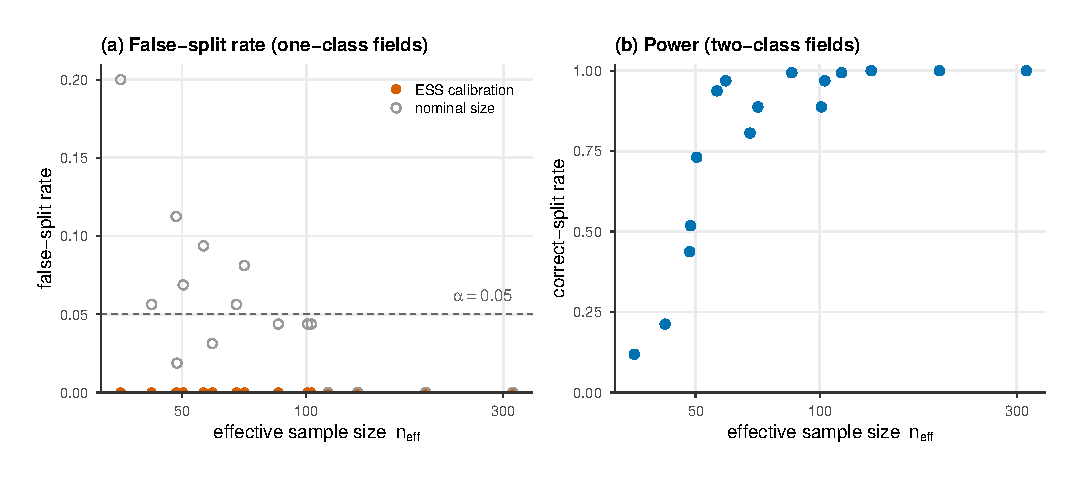
\includegraphics[width=\linewidth]{figures/level}
\caption{Direct validation of the effective-sample-size calibration on a single
homogeneity decision, $160$ realisations per cell. (a) On one-class Gaussian
fields the false-split rate of the calibrated test stays at $0.00$, at or below
the nominal $\alpha=0.05$, across effective sample sizes from $35$ to over $300$;
calibrating at the nominal size instead exceeds $\alpha$ (open symbols). (b) On
two-class fields \revtext{at separation $\delta=3$} the power rises with
$\neff$ to one, so the level is not the trivial conservatism of a test that
never rejects\revtext{; the curve is specific to that separation and moves with
it}.}
\label{fig:level}
\end{figure}

\subsection{Computational considerations}\label{subsec:complexity}

The range estimator \eqref{eq:areamed} costs one fast Fourier transform per
tile, $O(N\log N)$ in total \citep{CooleyTukey1965}. Each visited node runs one
$2$-means fit, of cost $O(n_C p)$ per iteration with mini-batch updates
\citep{Sculley2010}, and one dip evaluation, $O(n_C\log n_C)$
after sorting the projection \citep{HartiganHartigan1985}; the Monte Carlo quantiles
$q_{1-\alpha}(\cdot)$ are computed once per effective-size bucket and reused.
As the recursion visits each pixel in $O(\hat K)$ nodes, one ensemble member is
near-linear in $N$, and the $B$ members are independent and trivially parallel.
The procedure therefore scales to full scenes;
Section~\ref{subsec:timing} reports timings confirming a near-linear empirical
exponent and a memory footprint a small multiple of the data, together with a
constant-factor advantage over the gap statistic, whose reference replicates
multiply its cost.

\section{Simulation study}\label{sec:simulation}

We assess the procedure on synthetic scenes with known ground truth, where the
number of classes, the strength of spatial autocorrelation, the presence of a
trend, and the class separability are all controlled. The design isolates the
two failure modes of Section~\ref{subsec:null}, autocorrelation and
large-scale drift, and lets us measure how far the calibration keeps
the recursion from splitting, by counting how often each method
recovers a single class when the scene contains exactly one.

\subsection{Generative model}\label{subsec:design}

All scenes live on a $96\times96$ lattice with $p=6$ bands. The elementary
building block is a unit-variance Gaussian random field
$g_\sigma$, obtained by convolving Gaussian white noise with an isotropic
Gaussian kernel of bandwidth $\sigma$ (which sets the autocorrelation range)
and standardising. Four world types instantiate the decomposition
\eqref{eq:decomp}.
\revtext{The \emph{null} world ($K=1$) is pure autocorrelation with no discrete
structure: each band is an independent $g_\sigma$, with
$\sigma\in\{3,6,9\}$. The \emph{trend} world ($K=1$) has smooth large-scale
variation but no classes: each band is $\theta\,t(s)+0.4\,g_3(s)$, where $t$
is a standardised planar--bilinear polynomial surface and the trend amplitude
is $\theta\in\{1.5,3.0\}$. The \emph{structured} world
($K\in\{2,3,4,5\}$) embeds discrete classes in autocorrelated noise: a
contiguous label map is drawn as the pixelwise $\argmax$ of $K$ independent
fields $g_{\sigma_f}$, with $\sigma_f\in\{6,9\}$; class $k$ is assigned a mean
spectrum $\bm\mu_k\sim\mathcal N(\bm 0,\delta^2 I_p)$ with separation
$\delta\in\{2,3,4\}$; and a per-band autocorrelated noise $g_2$ is added.
Finally, the \emph{mixed} world ($K\in\{3,4\}$), the realistic case, combines
classes \emph{and} drift: a structured scene ($\delta=3$, $\sigma_f=6$) plus a
global polynomial trend of amplitude $\theta\in\{1.5,3.0\}$.}
The factorial of these settings yields $33$ cells ($3$ null, $2$ trend, $24$
structured, $4$ mixed); each cell is realised $15$ times with independent
seeds, for $495$ scenes in total.

\subsection{Methods and metrics}\label{subsec:methods}

We compare sixteen criteria. The decision rule of each is summarised
here\revtext{. Section~S2} of the supplementary material specifies every one in full,
including all tuning constants, the subsampling used by the indices that
require pairwise distances, and how the multiple-testing correction is applied,
and the released code reproduces each number with its seeds. Four are standard internal indices evaluated
over $K=1,\dots,8$ on MiniBatch $k$-means partitions: the gap
statistic \citep{Tibshirani2001} with eight uniform reference
datasets over the bounding box and the one-standard-error rule, the average
silhouette, Calinski--Harabasz, and Davies--Bouldin (each maximised over $K$,
\revtext{except Davies--Bouldin, which is minimised}). These four are the
original formulations, with no null model added by us\revtext{. The} null-calibrated
criteria in this benchmark are the autocorrelation-matched gap described
next, the Hennig--Lin variants,
and the proposed family, and in each case the null \revtext{was introduced by}
the work \revtext{that proposed} that calibration, not by the papers
that introduced the indices themselves. A fifth \revtext{criterion} is the most
direct spatial adaptation of an existing index, the \emph{gap with an
autocorrelated reference}\revtext{. It is} identical to the gap statistic except that the
eight reference datasets are drawn not uniformly over the bounding box but as
per-band Gaussian random fields whose $1/e$ range matches the tile-median
estimate of Section~\ref{subsec:range}\revtext{, and it uses} the same
one-standard-error rule\revtext{. The reference fields are} scaled to each band's
standard deviation as estimated from the scene itself, since no
deployable version of the criterion has access to the true value. \revtext{This
criterion} isolates how far
correcting only the reference's autocorrelation goes. (The \revtext{silhouette,
Calinski--Harabasz and Davies--Bouldin indices} cannot return
$K=1$ by construction, an asymmetry we return to below.) Two more are the
calibrated-validity-index method of \citet{HennigLin2015}, the procedure
ESS-Dip extends: the average silhouette width calibrated by parametric
bootstrap against a null model, run both with an \emph{i.i.d.} Gaussian null
(the autocorrelation-blind application) and with a \emph{spatial} null
(phase-\revtext{randomised} surrogates preserving each band's variogram, their
autocorrelation-aware variant adapted to the gridded setting). The
calibrated index is
$V(K)=\bigl(\mathrm{ASW}(K)-\overline{\mathrm{ASW}}_{\mathrm{null}}(K)\bigr)/
\mathrm{sd}_{\mathrm{null}}(K)$, computed from $B=20$ null datasets (scenes
subsampled to $1200$ pixels for tractability); $\hat K$ is the maximiser of
$V$ when $\max_K V(K)>1.96$ and $\hat K=1$ otherwise. An eighth baseline, plain \emph{dip-means}, applies the
same modality test at the nominal sample size, without the effective-sample-size
calibration, the local range, or the trend removal, isolating the contribution
of that spatial machinery. The ninth is the proposed method of
Section~\ref{sec:method}, denoted \textbf{ESS-Dip}:
Algorithm~\ref{alg:essdip} with the local within-class range
\eqref{eq:areamed}, adaptive trend removal \eqref{eq:detrendrule}, and a
$B=5$ ensemble; we fix $\alpha=0.05$, $\tau=0.25$, tile side $t=24$, and
$\nu=12$ throughout, with no per-scene tuning. The tenth, \textbf{ESS-Dip-R}, is
its recall-oriented variant: it calibrates the dip against the Gaussian null of
Assumption~\ref{ass:null} rather than the uniform least-favourable null, which is
less conservative and recovers more structure at the same specificity
(Section~\ref{subsec:simresults}). The \revtext{next} four are
ablations of ESS-Dip that disable one component each, to attribute the
contribution of every ingredient:
\emph{global range} (the $\ell^2$ range estimated over the whole image rather
than as a tile median); \emph{no trend removal}
($\tau=\infty$); \emph{forced trend removal} ($\tau=0$); and
\emph{declustering}, the precursor that subsamples the scene to one pixel per
decorrelation patch and applies the dip test to the thinned, approximately
independent sample. The fifteenth, \emph{SGS-Dip}, replaces the per-node
effective-sample-size calibration by the recursive Gaussian-simulation
reference \eqref{eq:sgstest} of Section~\ref{subsec:sgs} ($B=40$ simulations
per node); the sixteenth adds a Bonferroni multiple-testing correction to it.

Three metrics summarise performance. \emph{Specificity} is the fraction of
null and trend scenes (the $75$ scenes with $K=1$) for which $\hat K=1$; it is
the empirical analogue of Proposition~\ref{prop:fpr}. \emph{Exact-$K$ accuracy}
is the fraction of scenes with $\hat K=K_{\text{true}}$, reported separately
for the structured and mixed worlds, with the mean absolute error
$\mathrm{MAE}=\E\,\lvert\hat K-K_{\text{true}}\rvert$. The \emph{balanced
score} is the mean of specificity, structured accuracy and mixed accuracy, a
single figure that rewards methods strong across all three regimes rather than
in one.

\subsection{Results}\label{subsec:simresults}

Table~\ref{tab:bench} reports the three metrics; Figure~\ref{fig:bench}
displays the specificity--accuracy trade-off and the decay of accuracy with
the true number of classes.

\begin{table}[t]
\centering
\caption{Performance over the $495$ synthetic scenes. Specificity is the
$\hat K{=}1$ rate on the $75$ class-free (null${+}$trend) scenes; accuracy is
the exact-$K$ rate. Best in each column in bold.}
\label{tab:bench}
\begin{tabular}{l c cc c c}
\toprule
 & Specificity & \multicolumn{2}{c}{Structured} & Mixed & Balanced\\
\cmidrule(lr){3-4}
Method & ($\hat K{=}1$) & Acc. & MAE & Acc. & score\\
\midrule
\multicolumn{6}{l}{\textit{Standard internal indices} \textit{(no spatial null)}}\\
Gap statistic            & 0.00 & \textbf{0.97} & \textbf{0.03} & 0.03 & 0.336\\
Silhouette               & 0.00 & 0.76 & 0.32 & 0.30 & 0.355\\
Calinski--Harabasz       & 0.00 & 0.85 & 0.18 & 0.40 & 0.418\\
Davies--Bouldin          & 0.00 & 0.70 & 0.41 & 0.20 & 0.299\\
\midrule
\multicolumn{6}{l}{\textit{Calibrated validity index} \citep{HennigLin2015}}\\
\quad i.i.d.\ null       & 0.00 & 0.67 & 0.42 & 0.17 & 0.280\\
\quad spatial null       & 0.80 & 0.72 & 0.38 & 0.17 & 0.561\\
\midrule
\multicolumn{6}{l}{\textit{Spatial adaptation of an existing index}}\\
Gap (autocorrelated ref.) & 0.21 & \textbf{0.97} & 0.04 & 0.10 & 0.427\\
\midrule
\multicolumn{6}{l}{\textit{Modality test without spatial calibration}}\\
Dip-means (nominal)      & 0.52 & 0.92 & 0.09 & 0.02 & 0.486\\
\midrule
\multicolumn{6}{l}{\textit{Proposed}}\\
ESS-Dip                  & \textbf{1.00} & 0.81 & 0.35 & 0.50 & 0.771\\
ESS-Dip-R (recall)       & \textbf{1.00} & 0.89 & 0.19 & \textbf{0.72} & \textbf{0.868}\\
\midrule
\multicolumn{6}{l}{\textit{Ablations of ESS-Dip}}\\
\quad global range       & 1.00 & 0.63 & 0.87 & 0.28 & 0.638\\
\quad no trend removal   & 1.00 & 0.63 & 0.89 & 0.13 & 0.587\\
\quad forced trend removal & 1.00 & 0.19 & 1.95 & 0.30 & 0.498\\
\quad declustering       & 1.00 & 0.63 & 0.83 & 0.08 & 0.572\\
\midrule
\multicolumn{6}{l}{\textit{Exact reference as a recursive estimator}}\\
SGS-Dip                  & 0.85 & 0.49 & 0.91 & 0.27 & 0.535\\
\quad + multiple-testing correction & 0.99 & 0.79 & 0.26 & 0.35 & 0.710\\
\bottomrule
\end{tabular}
\end{table}

\begin{figure}[t]
\centering
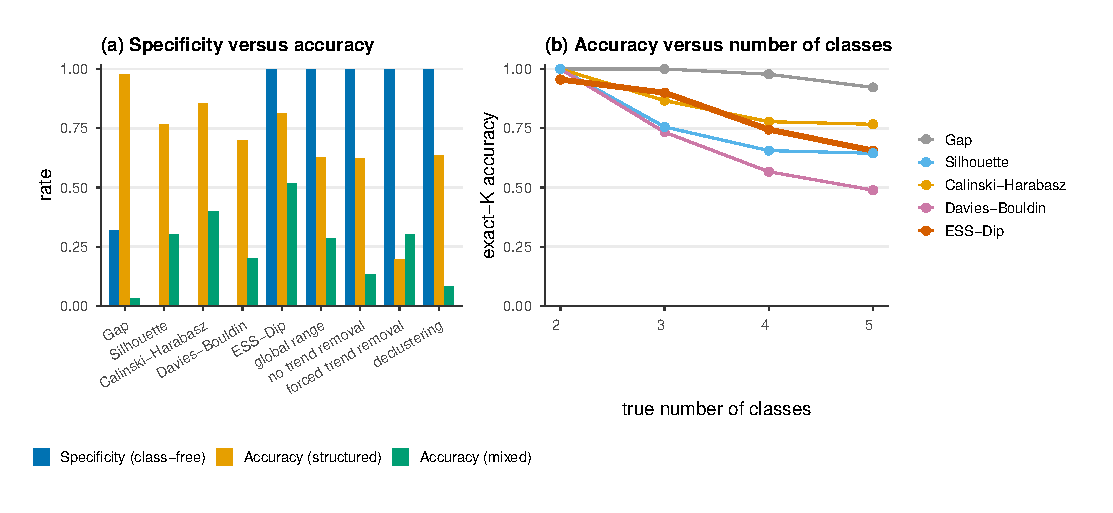
\includegraphics[width=\linewidth]{figures/benchmark}
\caption{Left: specificity (class-free scenes) against exact-$K$ accuracy on
structured and mixed scenes, by method. \revtext{Of the methods shown, only
ESS-Dip and its ablations attain unit specificity, and among them ESS-Dip
recovers the most structure.} Right: exact-$K$
accuracy versus the true number of classes on structured scenes. \revtext{For
legibility, the panels show the four standard indices, ESS-Dip and its
ablations; ESS-Dip-R and the} calibrated-validity-index and Gaussian-simulation methods of
Table~\ref{tab:bench} are omitted.}
\label{fig:bench}
\end{figure}

\paragraph{Standard indices report classes on every class-free scene.}
On the $75$ class-free scenes\revtext{,} every standard index reports spurious structure:
the $\hat K{=}1$ rate is $0.00$ for all four. The failure is severe, not
marginal: the gap statistic returns\revtext{, on average, $\hat K=7.7$} classes on
fields generated without any, and the silhouette, Calinski--Harabasz and
Davies--Bouldin indices average $2.9$, $3.6$ and $4.1$\revtext{, respectively}. This is the
over-detection anticipated in Section~\ref{subsec:null}, now quantified: under
spatial autocorrelation\revtext{,} an independence null cannot recognise the absence of
discrete structure in the sense of \eqref{eq:decomp}. Nor is the failure repaired by the simplest spatial
correction: the gap with an autocorrelation-matched reference \revtext{raises}
specificity only to $0.21$, because matching the reference's autocorrelation
addresses one of the two failure modes but not the other, the smooth drift.
On trend scenes\revtext{,} its reference fields carry no drift\revtext{,} and the criterion reads
the gradient as structure ($\hat K\approx7$ on average)\revtext{; in} the mixed
regime\revtext{,} its accuracy collapses to $0.10$\revtext{, and} its balanced score, $0.427$, \revtext{lies} far
below \revtext{that of} the proposed family. Fixing the reference is not enough\revtext{:} \revtext{both} the
dispersion statistic itself and the trend must be addressed.

\paragraph{The proposed family leaves the class-free scenes undivided.}
Every member of the proposed family\revtext{ (}ESS-Dip and all four ablations\revtext{)}
attains specificity $1.00$: in $75$ out of $75$ class-free scenes\revtext{,} it returns a
single class. This is the empirical content of Proposition~\ref{prop:fpr}, and
it holds whether the class-free scene is stationary (null) or carries a smooth
drift (trend), confirming that the effective-sample-size calibration and the
adaptive detrending together neutralise both failure modes.

\paragraph{Specificity does not cost competitiveness.}
On the structured scenes\revtext{,} the gap statistic is \revtext{the} most accurate
($0.97$): with well-separated classes and an aligned null\revtext{,} it is hard to beat,
and we do not \revtext{beat it}. ESS-Dip reaches $0.81$, ahead of the silhouette ($0.76$)
\revtext{and} Davies--Bouldin ($0.70$) and close to Calinski--Harabasz ($0.85$), while being
the \emph{only} \revtext{one of these} \revtext{methods} with non-zero specificity. On the realistic mixed
scenes\revtext{,} ESS-Dip reaches $0.50$, ahead of every standard index ($0.40$ for the
best), because the adaptive detrending removes the drift that \revtext{causes them to collapse}.
The recall variant ESS-Dip-R does better still: calibrating against the Gaussian
null of Assumption~\ref{ass:null} rather than the conservative uniform one, it
raises structured accuracy to $0.89$ and mixed accuracy to $0.72$ at the same
unit specificity, for a balanced score of $0.868$, the best of any method.
ESS-Dip itself scores $0.771$, already far above the next non-proposed method
($0.638$) and more than twice the best standard index ($0.418$). These synthetic
fields are Gaussian, so the model-matched ESS-Dip-R is favoured here; its
specificity and recall gains carry \revtext{over} to the real scenes of
Section~\ref{sec:application}. Standard indices that look strong on pure
structured scenes collapse once specificity is taken into account.

\paragraph{Comparison with the method that ESS-Dip extends.}
The calibrated-validity-index framework of \citet{HennigLin2015} is
instructive precisely because the present method generalises it. Applied with
an independence (i.i.d.) null\revtext{,} it inherits the over-detection of the standard
indices (specificity $0.00$, balanced score $0.280$), confirming that the
framework alone, without a spatial null, does not address the problem. With its
autocorrelation-aware (spatial) null\revtext{,} it recovers much of the lost specificity
($0.80$) and a comparable structured accuracy ($0.72$), a clear vindication of
its central idea. Two differences remain, and they are the contribution of this
paper. First, its specificity, at $0.80$, still admits one class-free scene in
five as clustered, where\revtext{as} the within-class calibration of ESS-Dip admits none.
Second, and decisively, on the mixed regime\revtext{,} its accuracy is only $0.17$,
no better than the i.i.d.\ variant and far below ESS-Dip's $0.50$, because a
phase-\revtext{randomised} null preserves the trend along with the autocorrelation and so
cannot separate a smooth drift from discrete classes. The explicit
trend--residual decomposition of Section~\ref{subsec:detrend}, absent from the
calibrated-index framework, is what closes this gap. This comparison is
insensitive to the significance threshold\revtext{. The} value used, $V>1.96$ (the
one-sided $2.5\%$ level for the calibrated index under approximate normality),
and the alternatives $V>1.64$ and $V>2.33$ all leave the conclusion intact\revtext{.
At} every threshold\revtext{,} the i.i.d.\ null fails \revtext{on} specificity ($0.00$), and the spatial
null controls specificity ($0.77$--$0.83$) but not the mixed regime
($\le0.08$). Figure~\ref{fig:recover} makes the mixed-scene
behaviour concrete on one realisation: the gap statistic and the Hennig--Lin
null fragment the scene into six and eight clusters\revtext{, respectively}, whereas ESS-Dip recovers
the three true classes.

\begin{figure}[t]
\centering
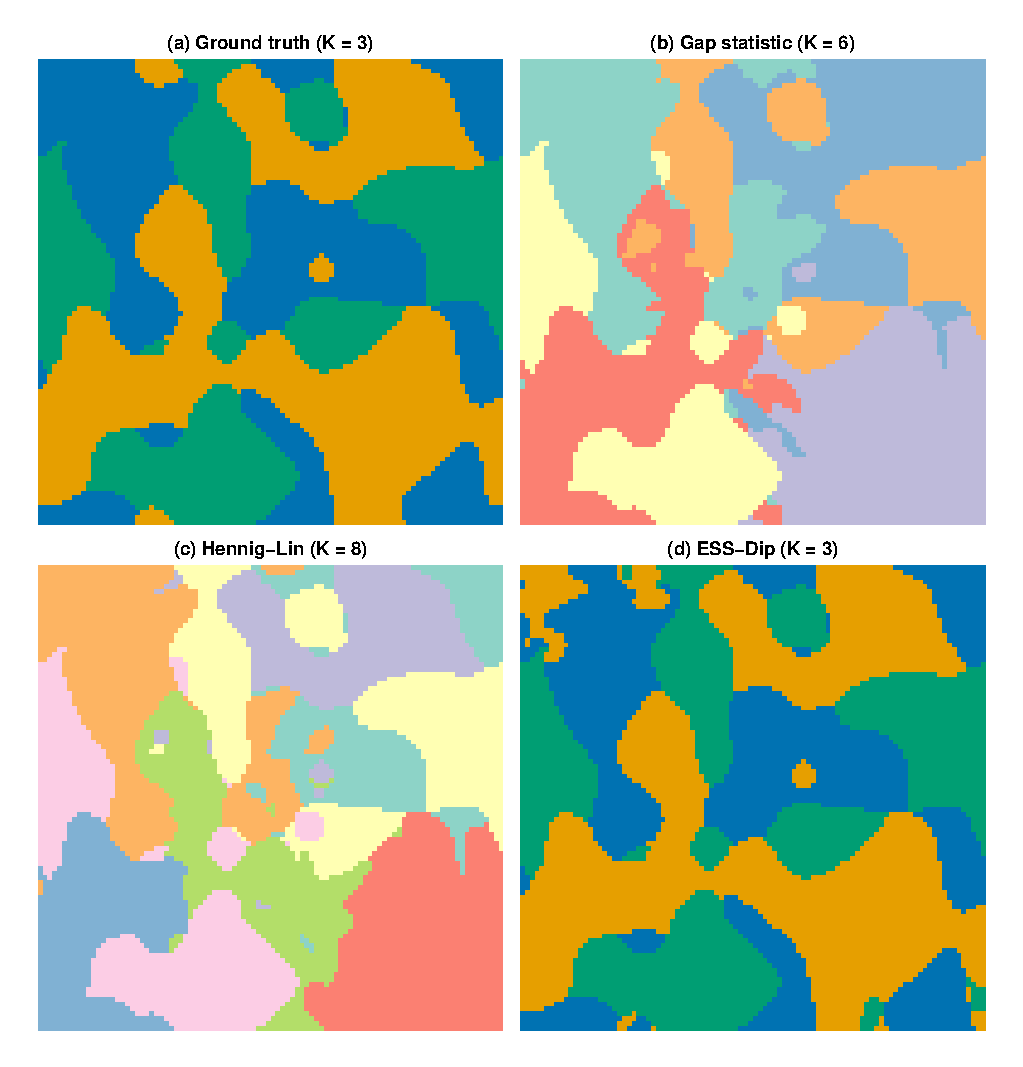
\includegraphics[width=\linewidth]{figures/recover}
\caption{Recovery on a representative mixed scene (three classes plus a smooth
trend). The gap statistic over-segments into six clusters (b) and the
Hennig--Lin spatial null into eight (c), both reading the trend and the
within-class autocorrelation as extra structure; ESS-Dip removes the trend and
calibrates to the effective sample size, recovering the three true classes (d),
whose partition matches the ground truth (a). Cluster colours in (b) and (c)
are arbitrary; in (a) and (d) they are matched, so a correct recovery
reproduces the colours of panel (a).}
\label{fig:recover}
\end{figure}

\subsection{Ablation}\label{subsec:ablation}

The ablations isolate where ESS-Dip's accuracy comes from
(Table~\ref{tab:bench}, lower block). The single largest contribution is the
\emph{local within-class range} of Section~\ref{subsec:range}: replacing it \revtext{with}
a scene-wide range \revtext{lowers} structured accuracy from $0.81$ to $0.63$ and mixed
accuracy from $0.50$ to $0.28$\revtext{, while leaving specificity untouched}. This confirms the diagnosis of
Section~\ref{subsec:range}\revtext{:} a global range conflates the between-class
mosaic with the within-class scale, inflating $\ell$, collapsing $\neff$, and
starving the test of power.
\emph{Adaptive} trend removal matters in both directions: forcing detrending on
every scene ($\tau=0$) destroys structured accuracy ($0.19$), because the
polynomial absorbs genuine between-class signal when no trend is present;
disabling it ($\tau=\infty$) \revtext{reduces} mixed accuracy \revtext{to $0.13$}, because an
unremoved drift inflates the range. Removing the drift \emph{only when present}
\revtext{preserves both} ($0.81$ structured, $0.50$ mixed). The declustering precursor,
which discards all but one pixel per patch, matches the others on specificity
but trails on accuracy ($0.08$ mixed), confirming the value of calibrating on
the full pixel set rather than thinning it. At the opposite extreme, plain
dip-means (Table~\ref{tab:bench}) removes the spatial apparatus entirely and
applies the dip at the nominal size: the modality signal alone recovers
structure well ($0.92$, second only to the gap statistic), but without the
effective-sample-size calibration its specificity falls to $0.52$, and without
trend removal its mixed accuracy collapses to $0.02$. The contribution of
ESS-Dip is therefore not the modality test, which is already strong, but the
spatial calibration and trend separation that turn it from a high-recall,
low-specificity splitter into a precision-controlled homogeneity test, at a
modest cost in structured recall ($0.92$ to $0.81$).

\subsection{Geostatistical reference and the effective-sample-size
approximation}\label{subsec:geostat-ref}

Section~\ref{subsec:range} offers, alongside the default $\ell^{2}$
proxy, a fitted variogram and its integral range, and
Section~\ref{subsec:sgs} offers the Gaussian-simulation reference
\eqref{eq:sgstest} in place of the effective-sample-size shortcut. Section~S4
of the supplementary material compares all three, and reports two findings
used elsewhere in this paper. First, as a single homogeneity test on a full
rectangular domain\revtext{,} the simulation reference decides correctly on every world,
accepting homogeneity on the class-free ones ($p=0.35$, $0.46$) and rejecting
it where classes are present ($p<10^{-3}$)\revtext{; this} is the assumption-light check
referred to in Section~\ref{subsec:prop}\revtext{. The} mean-based integral range,
however, is some three times larger than $\ell^{2}$ on these fields and so
loses recall, which is why the proxy is the default. Second, promoting the
simulation reference to a recursive estimator does not pay\revtext{. Without} a
multiple-testing correction\revtext{,} it over-splits (specificity $0.85$, balanced score
$0.535$)\revtext{; with} a Bonferroni correction\revtext{,} it becomes competitive on controlled
fields (balanced score $0.710$ against ESS-Dip's $0.771$)\revtext{; and} on real imagery\revtext{,}
its per-node variogram, fitted on irregular non-rectangular supports, leaves it
behind (Section~\ref{subsec:realspec})\revtext{. Moreover, it requires} $M$ simulations per node\revtext{,} against the
cached near-linear cost of \eqref{eq:test}. The apparent paradox that a
conservative correction raises accuracy is resolved in Section~S4: the
correction lowers $\hat K$ in every world, and accuracy rises because the
uncorrected recursion overshoots.

\subsection{Computational performance}\label{subsec:timing}

Figure~\ref{fig:timing} reports single-threaded wall-clock time on structured
scenes. Across image sizes from $\sim\!2{,}300$ to $\sim\!66{,}000$ pixels,
ESS-Dip scales with an empirical exponent
$\mathrm{d}\log t/\mathrm{d}\log N = 0.86$ (panel~a)\revtext{, which is} near-linear \revtext{and} consistent
with Section~\ref{subsec:complexity}, and is a constant factor (about
$1.2$--$2\times$) faster than the gap statistic, which scales similarly but
carries the overhead of its reference replicates. Cost grows sub-linearly with
the band count $p$ (panel~b: \revtext{from} $0.31$\,s at $p=3$ to $1.02$\,s at $p=40$, at
$N=128^2$). Peak memory \revtext{for a} $256\times256\times6$ \revtext{cube} is $8.9$\,MB, about three times
the input cube, so the method is memory-light at scene scale. The exact
Gaussian-simulation homogeneity test \eqref{eq:sgstest} with $B=120$ costs
$0.10$--$0.34$\,s over the same sizes\revtext{. This is} comparable to a single ESS-Dip
evaluation\revtext{ because} it concerns \revtext{a single} node; a fully recursive simulation null would
multiply this by the number of nodes, which is the cost the
effective-sample-size calibration is designed to avoid.

\begin{figure}[t]
\centering
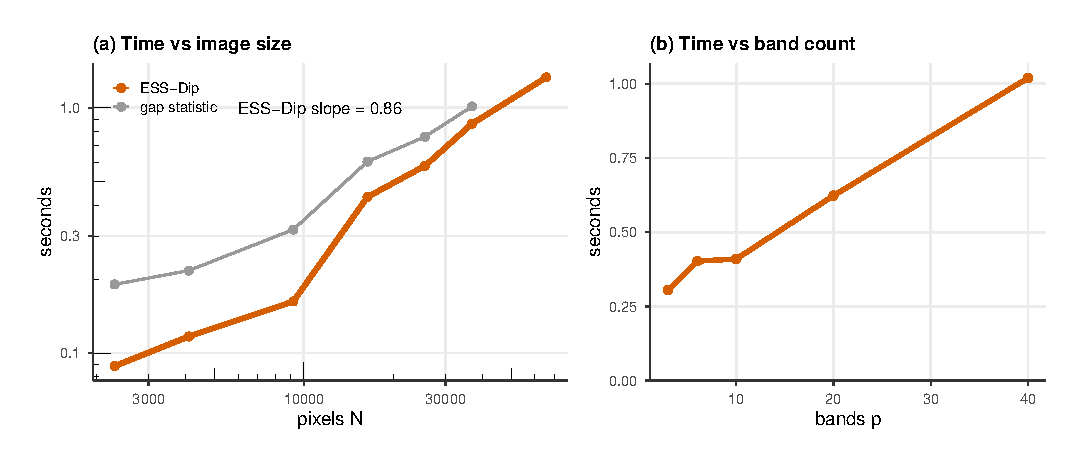
\includegraphics[width=\linewidth]{figures/timing}
\caption{Computational performance (single-threaded). (a) Wall-clock time
versus pixel count $N$ on a log--log scale, with the fitted ESS-Dip scaling
exponent; (b) time versus band count $p$ at $N=128^2$.}
\label{fig:timing}
\end{figure}

\subsection{Robustness to anisotropy}\label{subsec:aniso}

The decorrelation area \eqref{eq:areamed} is estimated from a radially averaged
(isotropic) variogram, yet directional autocorrelation does not degrade the
method. On null and structured worlds whose within-class range differs by a
factor of up to eight between the two axes, ESS-Dip retains specificity $1.00$
and structured accuracy $1.00$ at every anisotropy ratio tested ($1,2,4,8$),
whereas the gap statistic's specificity on the same class-free fields falls from
$0.88$ to $0.12$ as the field elongates. The isotropic scalar is thus an
adequate summary even under marked anisotropy\revtext{, because} the modality signal it feeds
\revtext{is} direction-agnostic\revtext{;} a fully anisotropic variogram
(Section~\ref{sec:discussion}) is a refinement rather than a necessity.

\subsection{Robustness to misestimation of the range}\label{subsec:misspec}

The calibration consumes a single estimated scale, so the practical question
is how much error in that scale the test tolerates. We answer it directly\revtext{. The}
locally estimated range $\ell$ is multiplied by a factor
$f\in\{\tfrac14,\tfrac12,\tfrac34,1,\tfrac32,2,4\}$ (the decorrelation area
scales as $f^2$)\revtext{,} and the full pipeline is re-run with the perturbed value\revtext{ on}
the null world (specificity) and on the structured world with $K=4$
(recovery), \revtext{with} $15$ paired scenes each. Table~\ref{tab:misspec} reports the
exact values\revtext{,} and Figure~\ref{fig:misspec} the response curves. The level is essentially indifferent to the error: overestimating the
range only makes the test more conservative, and even a four-fold
\emph{under}estimate, which inflates the effective sample size sixteen-fold,
raises the false-split rate merely to $0.07$, near the nominal $\alpha$,
because the least-favourable uniform calibration absorbs most of the slack
(Remark~\ref{rem:prop}). Recovery is asymmetric in the opposite direction\revtext{.} \revtext{It}
survives underestimation unharmed (full recovery at $f=\tfrac14$) and degrades
only under overestimation, retaining $\hat K=4$ in $73\%$ of scenes at
$f=\tfrac32$ and collapsing to no splits at $f=4$, where the effective sample
size falls below the testable minimum. The deployed estimator therefore \revtext{lies}
on the benign side of both asymmetries\revtext{.} \revtext{Errors} of up to a factor of two in the
range move the operating point along the precision--recall curve rather than
breaking the calibration, and the failure mode of a gross overestimate is
silence, not invention.

\begin{table}[t]
\centering
\caption{Sensitivity of the deployed pipeline to a multiplicative error $f$ in
the estimated range ($15$ paired scenes per world; the decorrelation area
scales as $f^2$). Each entry is an average over those $15$ scenes: the
first row gives the proportion on which the one-class world was divided at all
($\hat K>1$), the second the mean of $\hat K$ over the four-class world, and
the third the proportion of that world on which $\hat K$ equalled the true
$K=4$. $f<1$ underestimates the range (inflates $\neff$); $f>1$ overestimates
it.}
\label{tab:misspec}
\begin{tabular}{l ccccccc}
\toprule
Range factor $f$ & $1/4$ & $1/2$ & $3/4$ & $1$ & $3/2$ & $2$ & $4$\\
\midrule
Null world: false-split rate      & $0.07$ & $0.00$ & $0.00$ & $0.00$ & $0.00$ & $0.00$ & $0.00$\\
Structured ($K{=}4$): mean $\hat K$ & $4.00$ & $3.93$ & $3.93$ & $3.80$ & $3.67$ & $2.80$ & $1.00$\\
Structured ($K{=}4$): $\Prob(\hat K{=}4)$ & $1.00$ & $0.93$ & $0.93$ & $0.80$ & $0.73$ & $0.47$ & $0.00$\\
\bottomrule
\end{tabular}
\end{table}

\begin{figure}[t]
\centering
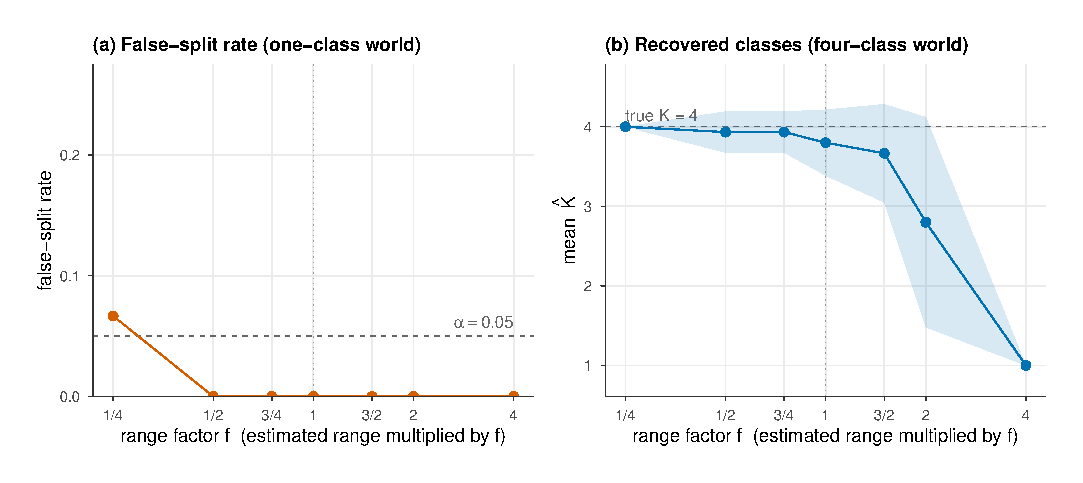
\includegraphics[width=\linewidth]{figures/misspec}
\caption{Robustness to a multiplicative error $f$ in the estimated range
(area scaling as $f^2$; dotted line marks the unperturbed estimate). (a)~The
false-split rate on the one-class world stays at zero under any overestimate
and reaches only $0.07$, near the nominal $\alpha$, under a four-fold
underestimate. (b)~Recovery on the four-class world (mean $\hat K\pm1$~sd)
survives underestimation unharmed and degrades only under overestimation,
collapsing to silence ($\hat K=1$), never to invention.}
\label{fig:misspec}
\end{figure}

\subsection{Class imbalance}\label{subsec:imbalance}

The Sentinel-2 result (Section~\ref{subsec:realfull}) suggests that a dominant
class hides minorities; here we quantify how severe the imbalance must be.
Two-class scenes are generated with a contiguous minority class occupying a
controlled proportion $\pi\in\{0.50,0.30,0.20,0.10,0.05,0.02\}$ of the domain
(a Gaussian random field thresholded at its $(1-\pi)$ quantile, class means
drawn as in Section~\ref{subsec:design})\revtext{, with} $15$ replicates at each of two
separations ($\mathrm{sep}=3,4$)\revtext{. The replicates are} pooled, \revtext{and} the same scene \revtext{is} shown to every
method. Table~\ref{tab:imbalance} reports the minority-detection rate
$\Prob(\hat K\ge2)$ and the mean $\hat K$; Figure~\ref{fig:imbalance}
displays the degradation curves. ESS-Dip detects the minority
reliably down to $\pi=0.20$ ($0.90$), degrades at $\pi=0.10$ ($0.73$)\revtext{,} and is
blind \revtext{from} $\pi=0.05$ \revtext{downwards}; the recall variant ESS-Dip-R extends the reliable
regime to $\pi=0.10$ ($0.93$) and detects half the cases at $\pi=0.05$. The
mechanism is the calibration itself: a minority occupying proportion $\pi$
contributes a mode of mass $\pi$ to the projected distribution, and once
$\pi\,\neff$ falls to the order of the decorrelation area the excess mass is
indistinguishable from autocorrelated fluctuation. The apparent robustness of
the baselines at extreme imbalance is not creditable as detection: their
false-split rate on class-free scenes is near one (Table~\ref{tab:bench}), so
a reported $\hat K\ge2$ carries no evidence, and at $\pi=0.02$ the silhouette
returns $\hat K\approx3$ by fragmenting the majority class rather than
isolating the minority. As practical guidance\revtext{,} minorities below about a fifth
of the scene call for ESS-Dip-R, and minorities below a twentieth are beyond
the specificity-controlled family at this separation, a limitation
Section~\ref{sec:discussion} returns to.

\begin{table}[t]
\centering
\caption{Detection of a contiguous minority class of proportion $\pi$ (true
$K=2$; $30$ pooled scenes per cell, identical scenes across methods). For the
baselines, $\Prob(\hat K\ge2)$ overstates detection because their false-split
rate on class-free scenes is near one (Table~\ref{tab:bench}).}
\label{tab:imbalance}
\small
\begin{tabular}{c cc cc cc cc}
\toprule
 & \multicolumn{2}{c}{ESS-Dip} & \multicolumn{2}{c}{ESS-Dip-R}
 & \multicolumn{2}{c}{Gap statistic} & \multicolumn{2}{c}{Silhouette}\\
\cmidrule(lr){2-3}\cmidrule(lr){4-5}\cmidrule(lr){6-7}\cmidrule(lr){8-9}
$\pi$ & $\Prob(\hat K{\ge}2)$ & $\bar{\hat K}$
       & $\Prob(\hat K{\ge}2)$ & $\bar{\hat K}$
       & $\Prob(\hat K{\ge}2)$ & $\bar{\hat K}$
       & $\Prob(\hat K{\ge}2)$ & $\bar{\hat K}$\\
\midrule
$0.50$ & $0.97$ & $1.97$ & $0.97$ & $1.97$ & $1.00$ & $2.00$ & $1.00$ & $2.00$\\
$0.30$ & $1.00$ & $2.00$ & $1.00$ & $2.00$ & $1.00$ & $2.00$ & $1.00$ & $2.00$\\
$0.20$ & $0.90$ & $1.90$ & $1.00$ & $2.00$ & $1.00$ & $2.10$ & $1.00$ & $2.00$\\
$0.10$ & $0.73$ & $1.73$ & $0.93$ & $1.93$ & $0.97$ & $2.07$ & $1.00$ & $2.00$\\
$0.05$ & $0.00$ & $1.00$ & $0.50$ & $1.50$ & $0.87$ & $2.33$ & $1.00$ & $2.03$\\
$0.02$ & $0.00$ & $1.00$ & $0.00$ & $1.00$ & $0.40$ & $1.60$ & $1.00$ & $2.97$\\
\bottomrule
\end{tabular}
\end{table}

\begin{figure}[t]
\centering
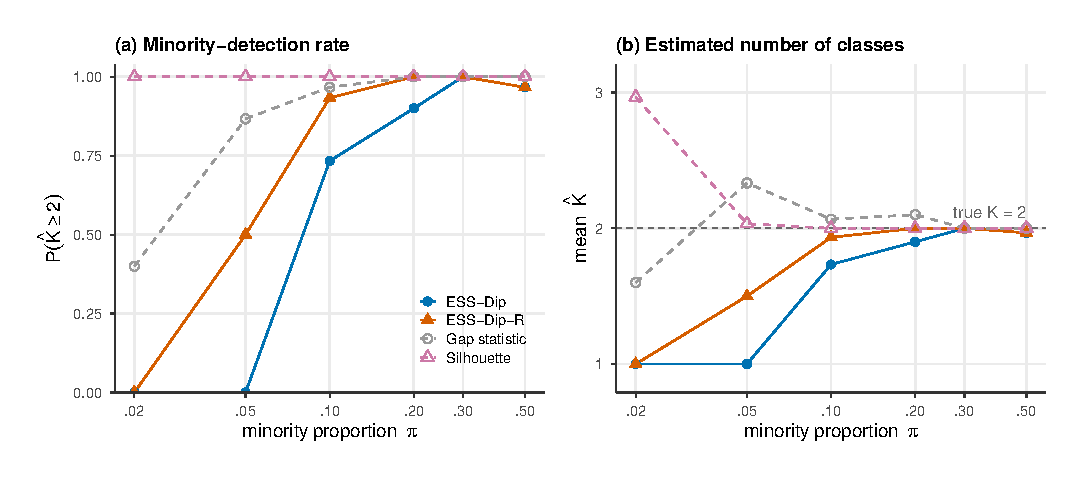
\includegraphics[width=\linewidth]{figures/imbalance}
\caption{Detection of a contiguous minority class of proportion $\pi$ (true
$K=2$; identical scenes across methods; dashed curves mark the baselines,
whose apparent detection is not creditable given their near-one false-split
rate on class-free scenes). (a)~ESS-Dip detects the minority reliably down to
$\pi=0.20$ and ESS-Dip-R extends the regime to $\pi=0.10$. (b)~At extreme
imbalance the silhouette reports $\hat K\approx3$ by fragmenting the
majority class, whereas the calibrated family degrades to silence
($\hat K=1$).}
\label{fig:imbalance}
\end{figure}

\section{Application to land-cover imagery}\label{sec:application}

We now turn to real scenes, where the question is no longer whether a method
recovers a known $K$ but whether it behaves sensibly on data with genuine
spatial autocorrelation, smooth illumination gradients, and spectrally
overlapping classes. We use three benchmarks spanning two sensing modalities
and report two experiments: a direct test of the specificity property of
Section~\ref{subsec:prop} on regions known to contain a single class, and a
full-scene estimate of the number of classes.

\subsection{Data and preprocessing}\label{subsec:data}

Two airborne hyperspectral scenes with per-pixel ground truth are used: the
\emph{Indian Pines} ($145\times145$, $200$ bands after removal of
water-absorption bands, $16$ classes; \citealp{Baumgardner2015}) and the
\emph{Salinas} scene ($512\times217$, $204$ bands, $16$ classes), both standard
in the classification literature. Each cube is standardised per band and
reduced by principal components to ten dimensions, retaining $95.5\%$ and
$99.6\%$ of the variance respectively. As a multispectral counterpart, the
common satellite setting, we use a $246\times237$ Sentinel-2 Level-2A scene
over the Po Valley with ten surface-reflectance bands (B02--B12), labelled by
the ESA WorldCover product \citep{Zanaga2022}; four classes exceed $1\%$ of the
scene (crop $83\%$, tree $9\%$, grass $5\%$, built $4\%$), so its nominal
number of classes is four. Bands are standardised; no dimensionality reduction
is needed.

\subsection{Within-class autocorrelation}\label{subsec:realvario}

The calibration presumes a within-class autocorrelation that is real,
estimable, and separable from the between-class mosaic; we verify all three on
the data. Averaging the radial empirical semivariogram of the first principal
component over pure single-class windows, each scene shows a well-defined
within-class structure (Figure~\ref{fig:variogram}): an exponential model fits
Indian Pines and Salinas (ranges $1.8$ and $1.4$ pixels) and a spherical model
fits Sentinel-2 (range $5.4$ pixels), with $1/e$ correlation lengths of two to
three pixels. The indicator-to-field integral-range ratio derived in
Section~\ref{subsec:sgs} holds on these real variograms:
$a_{\mathrm{int}}/a_I=1.51$, $1.54$ and $1.51$ for the three scenes, close to
the $1.45$ of the Gaussian fields. Local estimation separates the within-class
range from the scene scale: the tile-median range is $3$ to $4$ pixels, whereas
the scene-wide estimate, conflating the between-class mosaic, is three to
fifteen times larger ($14.5$ to $46$ pixels). The premise that most tiles fall
within a single class holds on the contiguous scenes ($62\%$ of Salinas and
Sentinel-2 tiles are single-class) and weakens on the fragmented Indian Pines
fields ($27\%$), where the tile median nonetheless recovers a within-class scale
($3.5$ against the $16$-pixel scene range), the robustness for which the median
is chosen.

\begin{figure}[t]
\centering
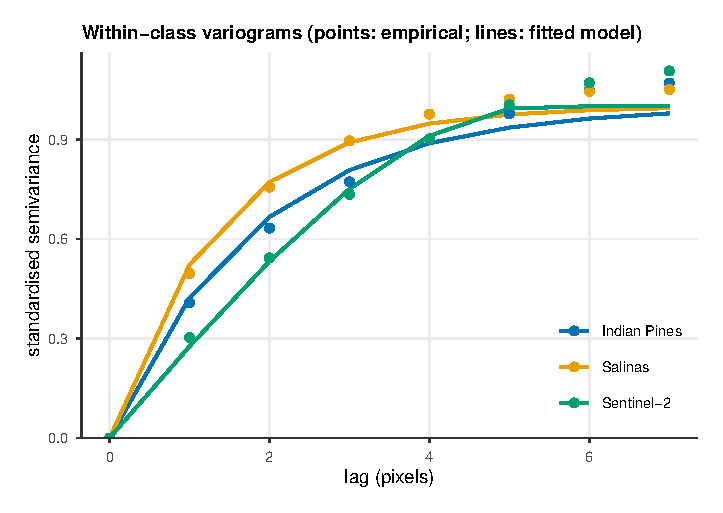
\includegraphics[width=0.62\linewidth]{figures/variogram}
\caption{Within-class variograms on the real scenes: the radial empirical
semivariogram of the first principal component (points), averaged over pure
single-class windows and standardised to unit sill, with the best-fitting
exponential, spherical or Gaussian model (lines). The within-class
autocorrelation the calibration relies on is real and has a well-defined range
on actual imagery.}
\label{fig:variogram}
\end{figure}

\subsection{Specificity on single-class regions}\label{subsec:realspec}

A region covered by a single land-cover class is the real-data analogue of the
null and trend worlds of Section~\ref{sec:simulation}: its pixels are
autocorrelated and spectrally variable (soil, moisture and illumination vary
within a crop field), yet the true number of classes is one. We extract all
$16\times16$ windows in which a single ground-truth class covers at least
$90\%$ of the pixels ($67$ windows across Indian Pines and Salinas, $60$ in the
Sentinel-2 scene, all of the dominant crop class), and record the number of
clusters each method reports. Table~\ref{tab:realspec} summarises the outcome;
the proposed-family ablations of Section~\ref{subsec:methods} all behave like
ESS-Dip here (specificity $\ge0.97$) and are omitted for brevity.

\begin{table}[t]
\centering
\caption{Number of clusters reported on single-class windows (true $K=1$).
A method calibrated for spatial autocorrelation should return $\hat K=1$.}
\label{tab:realspec}
\begin{tabular}{l cc cc}
\toprule
 & \multicolumn{2}{c}{Hyperspectral ($67$ win.)}
 & \multicolumn{2}{c}{Sentinel-2 ($60$ win.)}\\
\cmidrule(lr){2-3}\cmidrule(lr){4-5}
Method & $\hat K{=}1$ rate & mean $\hat K$ & $\hat K{=}1$ rate & mean $\hat K$\\
\midrule
Gap statistic       & 0.64 & 1.79 & 0.00 & 6.97\\
Silhouette          & 0.00 & 2.27 & 0.00 & 2.35\\
Calinski--Harabasz  & 0.00 & 2.70 & 0.00 & 3.20\\
Davies--Bouldin     & 0.00 & 3.37 & 0.00 & 2.62\\
\midrule
Hennig--Lin (spatial) & 0.72 & 2.36 & 0.07 & 4.77\\
Dip-means (nominal)   & 0.84 & 1.24 & 0.63 & 1.55\\
\midrule
ESS-Dip             & \textbf{0.99} & \textbf{1.01} & \textbf{1.00} & \textbf{1.00}\\
ESS-Dip-R (recall)  & 0.99 & 1.01 & 1.00 & 1.00\\
\bottomrule
\end{tabular}
\end{table}

The simulation result reproduces on real imagery. The silhouette,
Calinski--Harabasz and Davies--Bouldin indices split a single real land-cover
class into two or more sub-clusters in \emph{every} window of both modalities;
the gap statistic does so in all but the cleanest hyperspectral windows
($\hat K{=}1$ rate $0.64$) and, on the multispectral crop fields, fragments a
single class into nearly seven on average. ESS-Dip identifies the region as a
single class in $99\%$ of the hyperspectral and $100\%$ of the multispectral
windows. The within-field spectral variability that the standard indices read
as structure is precisely what the effective-sample-size calibration discounts.
The two closer baselines confirm the attribution on real data: the Hennig--Lin
spatial null, calibrated for autocorrelation, improves on the standard indices
over the hyperspectral windows ($0.72$) but collapses on the crop-dominated
Sentinel-2 fields ($0.07$, mean $\hat K=4.8$), where within-field variation
defeats its phase-randomized reference; plain dip-means, the modality test
without the effective-sample-size calibration, reaches $0.84$ and $0.63$. Both
trail ESS-Dip's $0.99$ and $1.00$, isolating the contribution of the spatial
calibration on real imagery.
The result is not an artefact of the preprocessing: on the Indian Pines windows
ESS-Dip returns a single class in every window across principal-component
truncations from five to thirty components, window sides from $12$ to $24$
pixels, and purity thresholds from $0.85$ to $0.95$ (for those combinations that
yield windows). The recursive Gaussian-simulation estimator,
even with the multiple-testing correction of
Section~\ref{subsec:geostat-ref}, is less reliable here: it returns a single
class in $0.82$ of the hyperspectral and $0.98$ of the multispectral windows,
below ESS-Dip, because its per-node plug-in variogram degrades on real,
non-stationary support, the residual effect that the correction does not
remove.

\subsection{Full-scene estimation}\label{subsec:realfull}

Applied to an entire labelled scene, the methods estimate the number of
land-cover classes present (Table~\ref{tab:realfull}). Two caveats
frame the reading of the table. First, $\hat K$ estimates the number of
classes \emph{distinguishable from the autocorrelation null at the effective
sample size}, not the nominal label count; failing to reject does not certify
that finer labelled classes are absent, only that the data do not support them
against the null, so a testing-based $\hat K$ is conservative by
construction. Second, no criterion approaches
the nominal sixteen classes of the hyperspectral scenes: the labels include
many small, spectrally similar agricultural classes that are not separable
without supervision, and the best standard index reaches nine (the gap on
Salinas) while the others return two to six. ESS-Dip is deliberately
conservative, reporting two classes on Indian Pines and five on Salinas. On the
crop-dominated Sentinel-2 scene, where a single class covers $83\%$ of the
pixels, ESS-Dip returns that one dominant class, whereas the gap reports five.
The recall variant ESS-Dip-R recovers more where the structure is separable,
reporting eleven classes on Salinas at the same single-class-window specificity
(Table~\ref{tab:realspec}), while remaining conservative where it cannot help:
two on the spectrally overlapping Indian Pines and one on the imbalanced
Sentinel-2, which are limited by separability and dominance, not by the
calibration's conservatism.

\begin{table}[t]
\centering
\caption{Estimated number of classes on full scenes; the nominal number of
labelled classes is given in parentheses. The $\ge20$ entry marks the recursive
simulation estimator reaching its recursion cap without terminating.}
\label{tab:realfull}
\begin{tabular}{l ccc}
\toprule
Method & Indian Pines (16) & Salinas (16) & Sentinel-2 (4)\\
\midrule
Gap statistic       & 3 & 9 & 5\\
Silhouette          & 2 & 2 & 2\\
Calinski--Harabasz  & 2 & 6 & 3\\
Davies--Bouldin     & 2 & 6 & 2\\
ESS-Dip             & 2 & 5 & 1\\
ESS-Dip-R (recall)  & 2 & 11 & 1\\
SGS-Dip (corrected) & 2 & $\ge20$ & 6\\
\bottomrule
\end{tabular}
\end{table}

These full-scene figures should be read against the precision--recall
trade-off of Section~\ref{subsec:simresults}. Exhaustive recovery of many
overlapping classes from a single scene is beyond every criterion considered,
and the conservatism of ESS-Dip is the price of its specificity: a procedure
that refuses to invent structure will, on a scene dominated by one class or
composed of weakly separated ones, under-report rather than over-report. The
recursive simulation estimator errs in the opposite direction, over-detecting
to the imposed cap on Salinas and to six classes on the crop-dominated
Sentinel-2 scene even after the multiple-testing correction, the plug-in
variogram on the scene's irregular, non-stationary support compounding over a
full-scene recursion. We
regard the method's value as residing in that precision (it answers
reliably whether genuine class structure is present beyond spatial
autocorrelation) rather than in maximal class enumeration, and we return to
this distinction, and to ways of relaxing it, in Section~\ref{sec:discussion}.

The number of classes is only half the picture; the quality of the induced
partition completes it. Table~\ref{tab:realari} reports the adjusted Rand index
(ARI) and normalised mutual information (NMI) of each labelling against the
ground-truth map. Two things stand out. First, unsupervised recovery of these
partitions is hard for every method: no ARI exceeds $0.52$. Second, on the
multi-class hyperspectral scenes ESS-Dip's partition quality trails the
over-detecting gap statistic (Salinas ARI $0.32$ versus $0.52$), and on the
crop-dominated Sentinel-2 scene, where it returns a single class, its ARI is
zero. This is the partition-quality counterpart of the conservatism already
visible in the class counts: a precision-oriented test that refuses to split
does not, and is not meant to, maximise partition recovery. The numbers make
the trade-off explicit and reinforce the reading of ESS-Dip as a homogeneity
guard rather than a classifier.

\begin{table}[t]
\centering
\caption{Partition quality on the full scenes: adjusted Rand index (ARI) and
normalised mutual information (NMI) against the ground-truth land-cover map,
with the number of classes each method returns. Computed on labelled pixels.}
\label{tab:realari}
\begin{tabular}{l l c cc}
\toprule
Scene & Method & $\hat K$ & ARI & NMI\\
\midrule
Indian Pines & Gap statistic & 3 & 0.21 & 0.36\\
             & Silhouette    & 2 & 0.18 & 0.37\\
             & ESS-Dip       & 2 & 0.18 & 0.37\\
\midrule
Salinas      & Gap statistic & 9 & \textbf{0.52} & \textbf{0.71}\\
             & Silhouette    & 2 & 0.18 & 0.37\\
             & ESS-Dip       & 5 & 0.32 & 0.57\\
\midrule
Sentinel-2   & Gap statistic & 5 & 0.10 & 0.14\\
             & Silhouette    & 2 & 0.36 & 0.22\\
             & ESS-Dip       & 1 & 0.00 & 0.00\\
\bottomrule
\end{tabular}
\end{table}

\section{Discussion}\label{sec:discussion}

\paragraph{A precision-oriented criterion.}
The results of Sections~\ref{sec:simulation} and~\ref{sec:application} draw a
consistent picture across synthetic fields, hyperspectral scenes and
multispectral imagery: standard internal criteria are powerful at recovering
well-separated classes but cannot recognise their absence, whereas ESS-Dip
controls the false-split rate at the cost of recall when classes are many or
weakly separated. The two behaviours are not interchangeable failures of
calibration but the two ends of a deliberate trade-off. By referring the dip
statistic to the effective rather than the nominal sample size, the test is
made conservative in exact proportion to the information the autocorrelation
removes; the level $\alpha$ and the range $\ell$ are the knobs that set where on
the precision--recall curve the method sits. We have fixed them once, without
per-scene tuning, and the resulting operating point is one of high precision:
ESS-Dip answers reliably whether discrete structure is present \emph{beyond}
spatial autocorrelation, and is correspondingly cautious about enumerating
structure that the data do not independently support. For the analyst this is
the useful direction of error, a guard against the over-segmentation that
Section~\ref{subsec:realspec} documents for the standard indices, but it is
a genuine limitation when an exhaustive class inventory is the goal. \revtext{This
defines the method's natural role. It is not a stand-alone classifier (on real
multi-class scenes it under-reports) but a calibrated homogeneity test: a guard
placed before an unsupervised classification, or a stopping rule for a
region-growing or regionalisation procedure} (Section~\ref{subsec:bg-constrained}), where a
negative one can trust is worth more than an exhaustive but unreliable class
count.

\paragraph{Choosing within the family, and embedding it in practice.}
The two calibrations serve different users. The default ESS-Dip is the choice
when a false split is the costly error (a homogeneity guard before
classification, a stopping rule, a confirmatory analysis) and whenever the
within-class marginal may be non-Gaussian, since the uniform null is
distribution-free. ESS-Dip-R is the better general-purpose class enumerator
when approximate within-class Gaussianity is plausible, as it typically is
after per-band standardisation and principal-component reduction: it recovers
substantially more structure at the same measured specificity (eleven against
five classes on Salinas; balanced score $0.868$ against $0.771$). The
imbalance sweep of Section~\ref{subsec:imbalance} makes the boundary
quantitative: minority classes below about a fifth of the scene call for the
recall variant, and \revtext{those below a twentieth lie beyond the reach of
both}. Neither variant needs a pre-selected univariate feature: the projection
is part of the procedure\revtext{ and is computed in the full feature space.
What} the method does require is a space in which Euclidean geometry is
meaningful, so bands should be
standardised and strongly collinear cubes reduced by principal components
(we use ten throughout; Section~\ref{subsec:realspec} shows the results are
insensitive to truncations from five to thirty). Three embedding patterns
cover the practical uses: as a pre-test that decides whether any unsupervised
classification of a scene is warranted at all; as the stopping rule of a
divisive or region-growing procedure, including spatially constrained
clustering (Section~\ref{subsec:bg-constrained}); and as a post-hoc audit
that applies the homogeneity test within each cluster proposed by any
external algorithm, flagging the clusters the data do not support.

\paragraph{Relation to geostatistical null models.}
Assumption~\ref{ass:null} replaces the independence reference of the
gap statistic \revtext{with a unimodal Gaussian random field, and supplies such a
reference where the ratio indices have none. This field is} the continuous-field
counterpart of the spatial neutral models used in disease mapping \citep{Goovaerts2004} and
of Moran spectral randomization \citep{WagnerDray2015}. We realise it
implicitly, through the effective-sample-size calibration of the dip, rather
than by simulating reference fields. A more explicit route would calibrate the
statistic against an ensemble of sequential-Gaussian-simulation realisations
conditioned on the empirical variogram; this would relax the isotropy built
into our scalar range $\ell$ and accommodate anisotropic or nested
autocorrelation structures at the cost of the simulation effort. We see the
present scalar calibration and a full simulation-based null as two points on a
spectrum trading fidelity against computation, and the near-linear cost of the
former (Section~\ref{subsec:complexity}) as its principal practical advantage
on megapixel scenes. The choice of null also encodes an analytical
judgement rather than a universal standard: the family's reference declares
autocorrelated continuous variation to be non-structure, which is the right
convention for class counting, but applications in which smooth sub-structure
is itself of interest (gradients within a single cover type that an analyst
wishes to subdivide, say) should not demand that their clusters of interest
defeat an autocorrelation null.

\paragraph{Limitations.}
Four limitations bound the method's applicability. First, when many spectrally
overlapping classes coexist, as in the sixteen-class hyperspectral scenes, no
unsupervised criterion, ours included, approaches the nominal class count
(Section~\ref{subsec:realfull}); recovering such inventories requires
supervision or auxiliary information that an internal criterion cannot supply.
Second, strong class imbalance degrades recall: when one class dominates the
scene, as the crop class does in the Sentinel-2 image, the leading split
direction is governed by that majority and minority classes are not resolved.
Third, the false-split control of Proposition~\ref{prop:fpr} is an asymptotic
statement resting on the empirical-process hypothesis (C3) and a fixed
projection, not a finite-sample guarantee. Fourth, the $2$-means
split direction is matched to balanced, spherical groups rather than to
density modes: when modes carry very different variances, or more than two
classes coexist at a node, the proposed direction can fail to expose the
multimodality or can cut through a class. The recursion re-tests every child,
and a poor direction costs recall rather than level
(Section~\ref{subsec:dip}); mode-seeking or projection-pursuit directions are
the natural refinement of this heuristic.

\paragraph{Extensions.}
Each limitation suggests a direction. The recall-oriented variant ESS-Dip-R
realises one: trading the distribution-free uniform null for the model's
Gaussian one recovers more structure at the same specificity (eleven classes on
Salinas against five). Further recall could come from revisiting leaves at a
relaxed level, or \revtext{from} testing minority modes against the residual of the majority,
to mitigate the imbalance that bounds the Sentinel-2 result. Replacing the scalar range by an anisotropic variogram model, and
the uniform dip null by conditional simulation, would extend the calibration to
non-stationary autocorrelation\revtext{. Section~\ref{subsec:aniso} shows, however,
that the isotropic estimate is already robust to directional autocorrelation up
to an eight-fold anisotropy ratio in the scenarios simulated there.} The same effective-sample-size
correction applies, unchanged, to spatio-temporal stacks, where the
decorrelation ``area'' becomes a space--time volume. Finally, because our
contribution is a stopping rule rather than a partitioning constraint, it
composes naturally with spatially constrained clustering
(Section~\ref{subsec:bg-constrained}): the calibrated test could decide when a
\revtext{regionalisation} has produced as many regions as the data independently
support.

\section{Conclusions}\label{sec:conclusions}

Selecting the number of clusters on spatial data runs into a
property the standard criteria share: they take no account of the dependence
between observations, and so cannot separate grouping that reflects discrete
classes from grouping that autocorrelation alone produces. Under spatial
autocorrelation the gap statistic and the silhouette, Calinski--Harabasz and
Davies--Bouldin indices reported several classes on every field we simulated
with one, and divided single land-cover regions on real imagery.

We have proposed a remedy framed in geostatistical terms. \revtext{The
problem is recast as a calibrated test of cluster homogeneity, which asks
whether a region carries multimodality in excess of spatial autocorrelation.
After removing a low-order trend whenever one is resolvable, ESS-Dip evaluates
the Hartigan dip along the locally optimal split direction and calibrates it
against the \emph{effective} sample size. That size is estimated from a
within-class autocorrelation range obtained by local range estimation.} For a stylised version
of the test we prove that the probability of dividing a homogeneous region
vanishes; the procedure runs in near-linear time. On a factorial
simulation with known ground truth it reaches unit specificity, and its recall
variant ESS-Dip-R attains the best balanced score of sixteen criteria at the
same specificity. \revtext{On the Indian Pines, Salinas and Sentinel-2
scenes, both variants} identify single land-cover regions as homogeneous where
the standard criteria do not. \revtext{The asymmetry between its two kinds of
error makes the family as suitable for use as a homogeneity guard or a stopping
rule for region-growing as for selecting the number of clusters, and the family
spans} a precision--recall axis from the conservative distribution-free null
to the higher-recall Gaussian one.

The broader message is that two long-standing tools of geostatistics,
the effective sample size and declustering, are what a clustering criterion
needs in order to answer this question on dependent data, and that the signal
which separates classes from autocorrelation is modality rather than
dispersion. All code and
data required to reproduce the simulation study and the applications are
released.

\section*{Code and data availability}
\addcontentsline{toc}{section}{Code and data availability}

All code required to reproduce the simulation study and the applications
(the synthetic-scene generators, the implementation of ESS-Dip and of every
baseline and ablation, the benchmark driver, and the figure scripts) is
openly available at \url{https://github.com/franciscoparrao/ess-dip}, released
under the MIT licence, and will be archived on Zenodo with a permanent DOI on
acceptance. The Indian Pines and Salinas hyperspectral scenes are the standard
public benchmarks \citep{Baumgardner2015}; the Sentinel-2 Level-2A imagery is
produced by the Copernicus programme and was accessed through the Microsoft
Planetary Computer; the land-cover reference is the ESA WorldCover product
\citep{Zanaga2022}. The synthetic scenes are generated deterministically by the
released code from the seeds reported in the repository.

\section*{Acknowledgements}
\addcontentsline{toc}{section}{Acknowledgements}

This work was carried out within the DICYT 2026--2027 postdoctoral fellowship
at the Universidad de Santiago de Chile (USACH), whose support the author
gratefully acknowledges. The author also thanks the Microsoft Planetary
Computer free-tier programme for access to the Sentinel-2 imagery used in the
application, and the providers of the public Indian Pines, Salinas and ESA
WorldCover benchmarks. This work relied on the open-source scientific Python
and R ecosystems.

\section*{Declarations}
\addcontentsline{toc}{section}{Declarations}

\paragraph{Funding.}
This research was supported by the DICYT 2026--2027 postdoctoral fellowship at
the Universidad de Santiago de Chile (USACH), project code 062619MC\_POSTDOC.

\paragraph{Conflict of interest.}
The author is the sole author of this work and declares that he has no
competing interests relevant to its content.

\paragraph{Data and code availability.}
All code and data required to reproduce the study are openly available, as
detailed in the section ``Code and data availability''.


\bibliography{refs}

\end{document}
